\documentclass[12pt]{article}
\usepackage[margin=1in]{geometry}
\usepackage{siunitx}
\usepackage{amssymb}
\usepackage{amsmath}
\usepackage{amsthm}
\usepackage{latexsym}
\usepackage{amsfonts}
\usepackage{graphicx,lscape,fancybox,shapepar,titletoc}
\usepackage{makecell}  % For text wrapping and truncation
\usepackage{xstring}   % To manually truncate text (if needed)
\usepackage{setspace}
\usepackage{fvextra}
\usepackage{booktabs}
\newcommand{\ra}[1]{\renewcommand{\arraystretch}{#1}}
\usepackage{newtxtt}
\usepackage{url}
\urlstyle{tt}
\usepackage{fullpage}
\usepackage{epstopdf}
\RequirePackage{xcolor}
\definecolor{CardinalRed}{cmyk}{0,1,0.65,0.34}
\usepackage[colorlinks=true, anchorcolor=CardinalRed, citecolor=CardinalRed,linkcolor=CardinalRed, breaklinks=true, urlcolor = CardinalRed]{hyperref}
\usepackage{tikz}
\usepackage{natbib}
\usepackage{array}
\setlength{\marginparwidth}{2cm}
\usepackage{todonotes}
\usepackage{xr}
\usepackage{caption}
\usepackage{subcaption}
\usepackage{lscape}
\usepackage[inline, shortlabels]{enumitem}
\usepackage{rotating}
\usepackage{longtable}
\usepackage{placeins}
%\usepackage{times}


% no indent for thanks
\usepackage{titling}
\settowidth{\thanksmarkwidth}{*}
\setlength{\thanksmargin}{-\thanksmarkwidth}

% no indent for footnotes
\usepackage[flushmargin]{footmisc}
\setlength{\footnotemargin}{2mm}

\RequirePackage[online]{threeparttable}

\newcolumntype{H}{>{\setbox0=\hbox\bgroup}c<{\egroup}@{}}

\setlength{\topmargin}{0pt} \setlength{\textheight}{8.5in}
\setlength{\parindent}{0.5in} \setlength{\textwidth}{6.5in}

\setlength{\topskip}{0in} \setlength{\headheight}{0in}
\setlength{\headsep}{0in} \setlength{\oddsidemargin}{0in}
\setlength{\evensidemargin}{0in}
\parskip=0in
\newtheorem{Theorem}{Theorem}
\newtheorem{acknowledgement}{Acknowledgement}
\newtheorem{algorithm}{Corollary}
\newtheorem{claim}{Claim}
\newtheorem{conclusion}{Conclusion}
\newtheorem{condition}{Condition}
\newtheorem{conjecture}{Conjecture}
\newtheorem{corollary}{Corollary}
\newtheorem{definition}{Definition}
\newtheorem{example}{Example}
\newtheorem{lemma}{Lemma}
\newtheorem{remark}{Remark}

\usepackage{listings}

\lstset{
  basicstyle=\ttfamily\small, % Use monospaced font
  breaklines=true,            % Enable line breaking
  breakatwhitespace=false,    % Allow breaking anywhere, not just at spaces
  numbers=left,               % Add line numbers on the left (optional)
  numberstyle=\tiny,          % Style for line numbers
  stepnumber=1,               % Line number step
  frame=single,               % Add a frame around the content
  showstringspaces=false,     % Don't show spaces as visible characters
  tabsize=2,                  % Set tab width
  xleftmargin=10pt,           % Add some left margin
  breakindent=0pt,             % Avoid excessive indentation after wrapping
  columns=fullflexible        % Ensure left-aligned and consistent spacing
}


\bibliographystyle{apsr}
\bibpunct{(}{)}{;}{a}{}{,}
\usetikzlibrary{arrows,positioning}
\tikzset{
    >=stealth',
    rec_a/.style={
           text width=11.5em,
           minimum height=3em,
           text centered},
    rec_b/.style={
           text width=9.5em,
           minimum height=2em,
           text centered},
    rec_c/.style={
           text width=5.5em,
           minimum height=2em,
           text centered},
    filled/.style={
            fill=circle area,
            draw=circle edge,
            thick},
    filled2/.style={
            fill=circle area2,
            draw=circle edge2,
            thick},
     outline/.style={
            draw=circle edge,
            thick},
     outline2/.style={
            draw=circle edge2}
}
\def\firstcircle{(0,0) circle (3.4cm)}
\def\secondcircle{(-.8,-.8) circle (1.8cm)}
\def\thirdcircle{(1,1) circle (.1cm)}

\colorlet{circle edge}{black!70}
\colorlet{circle area}{black!10}
\colorlet{circle area2}{white}
\colorlet{circle edge2}{white}

\def\Put(#1,#2)#3{\leavevmode\makebox(0,0){\put(#1,#2){#3}}}
\newcommand{\red}[1]{\textcolor{red}{#1}}
\externaldocument[]{anonymous}


%\vspace{-.25in}


%\renewcommand{\footnotelayout}{\onehalfspacing}
\renewcommand{\footnotesize}{\normalsize}
\setlength{\footnotesep}{1.25\baselineskip}
\setstretch{1.25}

\setcounter{table}{0}
\setcounter{equation}{0}
\setcounter{figure}{0}

\title{\bf The Credibility Revolution in Political Science
\thanks{\small Carolina Torreblanca, PDRI-DevLab Postdoctoral Fellow, Department of Political Science, University of Pennsylvania. Email: \href{mailto:catba@sas.upenn.edu}{catba@sas.upenn.edu}.  William Dinneen, Data Scientist. Email: \href{mailto:willdinneen@gmail.com}{willdinneen@gmail.com}. Guy Grossman, David M. Knott Professor of Global Politics, Department of Political Science and PDRI-DevLab, University of Pennsylvania, \emph{corresponding author}. Email: \href{mailto:ggros@upenn.edu}{ggros@upenn.edu}. Yiqing Xu, Assistant Professor, Department of Political Science, Stanford University. Email: \href{mailto:yiqingxu@stanford.edu}{yiqingxu@stanford.edu}. We thank Yunfei Chen, Ziyi Chen, Biman Yang, Jiawei Zou, and Honaminto E. Djohi for excellent research assistance.}}

\author{Carolina Torreblanca\\(UPenn) \and William Dinneen\\(Stanford) \and Guy Grossman\\(UPenn) \and  Yiqing Xu\\(Stanford)}


\date{\bigskip\today}

\begin{document}
  \maketitle
\thispagestyle{empty}
\setstretch{1}
\vspace{-2em}\begin{abstract}
\noindent How has the credibility revolution shaped political science? We address this question by classifying 91,632 articles published between 2003 and 2023 across 156 political science journals using large language models, focusing on research design, credibility-enhancing practices, and citation patterns. We find that design-based studies—those leveraging plausibly exogenous variation to justify causal claims—have become increasingly common and receive a citation premium. In contrast, model-based approaches that rely on strong modeling assumptions have declined. Yet the rise of design-based work is uneven: it is concentrated in top journals and among authors at highly ranked institutions, and it is driven primarily by the growth of survey experiments. Other credibility-enhancing practices that help reduce false positives and false negatives, such as placebo tests and power calculations, remain rare. Taken together, our findings point to substantial but selective change—more consistent with a partial reform than a revolution.
\end{abstract}

\newpage
\setstretch{1.75}
\setcounter{page}{1}

\section*{Introduction}\label{sec:intro}

Over the last two decades, political science has been influenced by what many describe as a credibility revolution: an intellectual movement advocating a change in how researchers conceptualize and conduct causal empirical scholarship \citep{angrist2010credibility, dunning2012natural, gerber2012field, morgan2014counterfactuals, samii2016, aronow2019foundations, blair2023research, SloughTyson2024, imbens2025comparing}. But how far has this revolution actually reshaped the field? In this paper, we examine whether and to what extent the credibility revolution movement has altered the landscape of empirical causal research in political science. 

As an epistemic movement that reshapes what researchers view as credible evidence when assessing causal claims, the credibility revolution carries transformative potential. Its intellectual core is a reconceptualization of causality. This reconceptualization encourages a shift away from model-based strategies---which often rely on strong functional form assumptions and implicit views of treatment assignment---toward design-based approaches that exploit features of treatment assignment and rest on explicit identification assumptions. Notably, this movement views credibility not solely as a consequence of adopting specific designs such as experiments or natural experiments. In addition, it proposes a clearer articulation of identification assumptions and supporting evidence through credibility-enhancing practices such as pre-analysis plans, power analyses, and placebo tests \citep{sekhon2009opiate}. %At the same time, critics have raised concerns about external validity and over-reliance on as-if-random designs, underscoring that research design and substantive relevance must be considered jointly. 

Whether, on balance, this movement has produced an epistemic revolution in political science depends on how widely and deeply these ideas have reshaped actual research practice. Quantifying the depth and breadth of the movement's influence presents two measurement challenges. The first is scope. What constitutes a sufficiently representative sample of political science to allow statements about the discipline as a whole? Previous research examining methodological changes in other social science disciplines has focused on elite journals or publishing outlets \citep[e.g., ][]{currie2020technology, goldsmith2024tracking}. However, the discipline extends far beyond these outlets, which may publish systematically different research than the rest of the field. Consequently, a systematic assessment of potential changes requires analyzing papers across multiple journal tiers over a substantial period. We address this by analyzing 91,632 articles from 156 political science journals spanning 2003--2023 using large language models (LLMs). This represents, to our knowledge, the most comprehensive analysis of political science research assembled to date.

The second challenge is operationalization. The credibility revolution is an intellectual movement that seeks to transform empirical research. Translating such ideas into concrete research decisions is not straightforward. What changes should we expect to observe if its ideas have taken hold? We focus on three dimensions where change should be evident: (1) the methodological approaches employed in quantitative political science papers, (2) the adoption of practices that enhance credibility beyond research design, and (3) the professional rewards these approaches receive relative to the approaches they aim to substitute.

We leverage advances in LLMs to classify our corpus along these dimensions. We begin by mapping papers by methodology and research goals, then narrow our focus to explanatory empirical quantitative papers—the subset most likely to be shaped by the credibility revolution. Within this subset, we distinguish between design-based approaches, which most straightforwardly embody the principles of the credibility revolution by leveraging features of the data-generating process for causal identification, and model-based approaches, which ground identification primarily in parametric or other modeling assumptions. We also code the use of several ancillary practices--- e.g., power analysis, and placebo tests---which have the potential to further buttress the credibility of causal claims made in quantitative papers.

We first assess the extent to which design-based empirical research has substituted model-based approaches in quantitative studies that aim to explain social phenomena. We find substantial, though uneven, substitution. Design-based methods increased from 15\% to 40\% of explanatory quantitative studies between 2003 and 2023, while model-based approaches declined from 57\% to 39\%. Notably, survey experiments, which narrowly identify the causal effect of information provision, accounted for 44\% of all design-based papers in 2023. Further, such replacement is primarily concentrated in top journals. Taken together, these patterns suggest that while a methodological shift has occurred, it remains partial and uneven: traditional strategies continue to play a central role in explanatory research, especially in lower-visibility outlets.

Second, we examine the adoption of practices that enhance credibility beyond research design. Such practices remain uncommon even among design-based studies. Pre-analysis plans and power analyses appear in only 6\% and 16\% of experimental papers, respectively, and placebo tests are reported in just 22\% of design-based observational studies. These patterns indicate that the credibility revolution’s influence beyond methodological substitution remains limited and has not yet produced broader shifts in research standards.

Third, we assess whether design-based research receives different professional rewards than model-based approaches. Descriptively, we find that design-based studies receive more citations than model-based papers, and this gap has widened over time. This citation premium has grown but now appears to have stabilized, suggesting that the discipline’s reward structure has shifted to favor more credible methods and may be reaching a new equilibrium.

Overall, we find evidence of a moderate influence of the credibility revolution. Design-based methods have grown while model-based approaches have declined, indicating an increase in quantitative research that aligns with the movement’s principles. Yet the movement's influence is neither wide nor deep. It is not wide for two reasons. First, much of political science lies outside the domain where the credibility revolution's lessons most directly apply: quantitative studies that seek to identify causal relationships. Thus, limits to the movement's reach partly reflect enduring methodological diversity in the discipline. Second, traditional model-based approaches remain deeply embedded in quantitative empirical explanatory research. 

The movement's reach is not deep in the sense that, even among scholars adopting design-based methods, broader credibility-enhancing practices remain rare, and the shift is driven largely by one approach—survey experiments, which accounted for nearly half of all design-based papers in 2023. In this light, the credibility revolution is best understood as a reform: a real but limited transformation, concentrated in relatively small—though not unimportant—segments of the discipline.

One might be tempted to infer from our results that political science research has become more credible because of this reform process. Design-based approaches have indeed become more prevalent, consistent with what proponents of the credibility revolution advocated. However, our analysis is descriptive, not prescriptive. It documents changes in how scholars conceptualize causality, how they justify causal claims, and what ancillary evidence they report in support of those claims, taking papers’ reporting at face value. We neither can nor intend to adjudicate whether identifying assumptions in any given paper are warranted, whether analyses were executed well, or whether specific findings are correct. There is no inherent hierarchy between the two approaches; credibility derives from the validity of assumptions and the quality of implementation. In any application, both design-based and model-based approaches may rest on defensible assumptions and be implemented well, or may be misspecified, poorly executed, and unconvincing. We therefore interpret the patterns we document as a shift in the conventions by which political scientists justify identification and present causal claims in print, not as evidence that published findings are now more likely to be correct.

Our paper builds on \citet{currie2020technology} and \citet{goldsmith2024tracking}, who quantify the credibility revolution movement in economics using papers published in elite journals and National Bureau of Economic Research (NBER) working papers series. A key limitation of these studies is that NBER affiliates do not represent the economics discipline as a whole. By contrast, we analyze articles from all political science journals with an impact factor above one, allowing us to examine the field well beyond the outlets targeted by scholars from elite institutions. 

We also extend work by \citet{garg2025causal}, who use LLMs to identify causal claims in economics, by systematically classifying design choices and transparency practices across an entire discipline, and complement recent large-scale diagnostic analyses of quantitative political science that evaluate the inferential properties of published research \citep{arelBundock2026underpowered}. Finally, our work contributes to a broader literature on how the credibility revolution has shaped political science, including patterns of knowledge production, graduate training and hiring, and the evolution of methodological norms~\citep{grossman2025political}.

\section*{The Credibility Revolution}\label{sec:ourapproach}

We use the term ``credibility revolution'' to refer to a broad movement in the social sciences that sought to change how empirical causal research is conducted and evaluated. As an epistemic project, it foregrounded the need for explicit and defensible identification assumptions in quantitative causal research and placed particular emphasis on theorizing about the data-generating processes when justifying causal comparisons \citep{morgan2014counterfactuals, imbens2015causal}. It emphasized the value of making identification strategies transparent and open to scrutiny, and of reducing reliance on modeling assumptions as the basis for causal claims when these are difficult to defend~\citep{aronow2019foundations, samii2016}.

Like many epistemic movements, the credibility revolution is broad, heterogeneous, and internally contested. Our aim is not to adjudicate its ``exact'' meaning, but to identify a core distinction that allows us to measure how empirical causal practice has changed in response to it. To that end, we adopt an analytically useful taxonomy that distinguishes between two broad approaches to empirical causal research. The taxonomy is imperfect --- methods associated with a design-based approach may combine elements of the model-based approach (e.g., difference-in-differences)--- but it captures a central difference in where causal identification is anchored: whether identification rests primarily on features of treatment assignment or on assumptions embedded in statistical models.

\begin{itemize}\itemsep0em
\item \emph{Design-based approaches} ground causal identification in features of the data-generating process that structure treatment assignment in a plausibly exogenous fashion, such as randomization, institutional rules, or policy thresholds. While estimation may rely on statistical models, the validity of causal claims is understood to rest primarily on assumptions about treatment assignment and counterfactual comparisons, rather than on functional-form or distributional assumptions. Natural experiments, randomized controlled trials, instrumental variables, regression discontinuity designs, and difference-in-differences designs are canonical examples.\footnote{In essence, the parallel trends assumption underlying difference-in-differences designs is a mean-independence assumption between the treatment and demeaned or first-differenced non-treated potential outcomes.}

\item \emph{Model-based approaches}, conversely, ground causal identification primarily on the correctness of parametric or statistical modeling assumptions---such as linearity, additivity, conditional independence, and distributional assumptions. In these approaches, causal interpretation hinges on the plausibility of modeling assumptions, which are often tied to theory or data structure, and may be plausible depending on the context. These assumptions are typically not anchored in an explicit claim about the treatment assignment process.
\end{itemize}

\section*{The Credibility Revolution and Political Science}\label{sec:ourapproach}

The credibility revolution began in applied microeconomics in the early 1990s, driven by studies that sought to exploit institutional rules, spatial policy changes, and quasi-random variation to identify causal effects \citep[e.g.,][]{angrist1991does,card1994minimumwage}. It built on earlier critiques that regression-based causal claims were often fragile to specification choices and sensitive to researcher degrees of freedom~\citep{leamer1983}, as well as program-evaluation evidence showing that conventional observational adjustments could diverge sharply from experimental benchmarks \citep{lalonde1986}. These contributions challenged prevailing practices that relied heavily on parametric regression models for causal interpretation, with causal claims resting largely on modeling choices. Researchers typically modeled the conditional expectation of an outcome using treatment variables and covariates (often without a clear distinction between the two) and then interpreted regression coefficients as causal effects. This practice placed a heavy burden on modeling assumptions, often without direct scrutiny of the underlying identification strategy.

These novel empirical developments built on formal frameworks for causal inference in statistics that emphasized explicit statements of identification assumptions. The Neyman–Rubin potential outcomes framework provided a common language for defining causal effects \citep{rubin1974, holland1986}, while the structural causal model and directed acyclic graph framework provided a graphical representation of causal assumptions~\citep{pearl2009Causality}. Additionally, related contributions formalized the assumptions underlying instrumental-variable designs and local average treatment effects \citep{imbens1994identification}. 

Several research designs became especially prominent within the movement. Difference-in-differences designs provided a flexible framework for exploiting policy changes and temporal variation \citep{card1994minimumwage}. Natural experiments leveraged institutional rules or geographic discontinuities to isolate plausibly exogenous variation in treatment assignment \citep{dell2010persistent}, while instrumental variable approaches addressed unobserved confounding under explicit exclusion assumptions \citep{acemoglu2001colonial}. Randomized controlled trials gained renewed attention for their transparency in identifying average treatment effects, and regression discontinuity designs offered credible identification in narrow windows around policy and electoral thresholds \citep{lee2008rd}. Despite differences in scope and assumptions, these designs share an emphasis on explicitly linking causal identification to features of the empirical context.

Political science absorbed these ideas, with some lag, through multiple channels. Early field experiments demonstrated the feasibility of randomized interventions in political settings \citep{gerber2000field, wantchekon2003clientelism}, while the synthesis of natural experiments in \citet{dunning2012natural} helped codify design-based reasoning within the discipline. Regression discontinuity designs became influential in electoral studies \citep{eggers2015validity}, and instrumental-variable approaches grounded in local average treatment effects gained traction in comparative and international research \citep{sovey2011instrumental}. Difference-in-differences designs also became increasingly common, particularly in studies of policy change~\citep{bechtel2011lasting}.

The diffusion of credibility-revolution ideas also coincided with increased attention to research practices intended to make empirical claims more transparent and, thereby, to increase the credibility of reported findings. Robustness checks, placebo tests, and sensitivity analyses became more common, alongside the spread of pre-analysis plans and data and code sharing. While transparency and reproducibility practices have distinct intellectual origins from design-based identification strategies, they similarly emphasize making assumptions and analytic choices visible, ensuring their soundness, and thereby making them more credible.

These developments have not gone uncontested. A growing body of scholarship has emphasized the limitations and trade-offs of design-based approaches. One critique concerns the locality of estimands: credible causal estimates often pertain to narrow subpopulations or institutional settings, limiting their theoretical and policy relevance \citep[e.g.,][]{heckman1995randomization}. A related concern is that the focus on quasi-random variation can narrow the scope of inquiry. In privileging what can be credibly identified, researchers may sideline substantively central but historically contingent processes---such as democratization or state formation---that resist design-based identification~\citep{mahoney2006tale}.

Other critiques highlight the tension between credible identification and interpretation. Even when causal effects are well identified, their meaning often rests on untested assumptions about mechanisms, scope conditions, and counterfactual relevance. These concerns are especially salient when generalizing from localized interventions to broader theories of political behavior or institutional change~\citep{findley2021external}. %In parallel, scholars have questioned the robustness of the assumptions underlying experimental designs~\citep{deaton2018understanding}. 
Taken together, these critiques underscore that the credibility revolution reflects a specific epistemological orientation—one that prioritizes internal validity and research design rigor—but does not resolve longstanding tensions among identification, explanation, and generalization in empirical political science.

\subsection*{On Survey Experiments}\label{sec:surveys}

Survey experiments occupy an ambiguous position in the genealogy of the credibility revolution. They emerge from a distinct epistemic lineage---rooted in psychology and behavioral science---that predates the methodological debates over causal identification that animated applied microeconomics in the 1990s and 2000s. Many early survey experiments were developed primarily as tools for measurement and elicitation, designed to probe latent attitudes, beliefs, or cognitive processes~\citep{mutz2011population}. In this tradition, the goal was not necessarily to estimate the causal effects of real-world political interventions, but rather to improve our understanding of the psychological mechanisms underlying political behavior. In this respect, survey experiments are not direct descendants of the credibility revolution as it coalesced around the identification of causal effects in field settings.

At the same time, survey experiments are experiments and, in that sense, they do resonate with the credibility revolution's emphasis on exogenous treatment assignment and transparency in the data-generating process. Yet the scope of the intervention in survey experiments is typically narrow: what is manipulated is information---delivered via vignettes, prompts, or framing---rather than political conditions, policies, or institutional arrangements themselves. This allows researchers to identify the causal effect of informational treatments in controlled environments. But the causal estimand often pertains to short-term attitudinal shifts in response to textual stimuli, rather than to behavioral or institutional change. As such, the causal effects identified are typically well-defined but substantively constrained, and their real-world implications can be difficult to trace~\citep{barabas2010survey}.

For these reasons, we classify survey experiments as part of the broader design-based category in our analyses, consistent with their widespread treatment in the discipline as causally identified research designs. At the same time, we recognize that their distinct origins and the limited manipulability of their treatments raise important questions about how they contribute to the goals of the credibility revolution. To reflect this duality, we present results both including and disaggregating survey experiments from other design-based approaches, allowing us to assess how their inclusion shapes broader inferences about methodological change in political science.

\section*{Quantifying the impact of the credibility revolution.} 

If the credibility revolution reshaped empirical practice in political science, its effects should be observable in how quantitative causal research is conducted, reported, and rewarded. We assess its impact along three dimensions: methodological choices, transparency practices, and professional recognition. First, we examine shifts in research design. To the extent that the credibility revolution influenced empirical practice, we would expect a move away from approaches that rely primarily on modeling assumptions and toward those that ground causal claims in identification strategies that leverage explicit features of the data generating process. Empirically, this should manifest as growth in the use of design-based methods relative to model-based approaches broadly.

Second, we evaluate changes in transparency (e.g., PAPs) and reporting practices (e.g., power calculations and placebo tests). While, as mentioned, these practices have distinct intellectual roots, they are now frequently bundled with credibility-revolution standards in contemporary empirical work~\citep{blair2023research} and their proponents emphasize their ability to lend credibility to causal claims~\citep{sekhon2009opiate}. If such practices have diffused beyond research design alone, we should observe increased adoption of practices that clarify identification assumptions and analytic decisions.

Third, we assess whether these methodological shifts are reflected in professional rewards. If standards of credible causal inference have changed within the discipline, research that employs design-based methods or associated transparency practices may receive greater recognition. We examine this by analyzing publication patterns and citation outcomes, testing whether design-based studies are systematically rewarded relative to model-based work, holding constant publication timing and venue.

\section*{Data and Measurements}\label{sec:data}

We evaluate these predictions using a corpus of political science research from the past two decades. In this section, we describe the data, key measurements, and methods used to construct these measures.

We began with a set of 188 journals identified by \href{https://clarivate.com}{Clarivate} as part of the political science discipline and having a Scientific Journal Rankings (SJR) score of at least one. This threshold roughly corresponds to the upper tier of the field in citation influence and focuses attention on outlets that sit near the center of political science's citation network. From this list, we removed journals for three distinct reasons: indexing (three journals not indexed in Scopus), quality control (three journals that lacked peer review), and language or format (seven journals that were not published in English and one listed as a book series). The resulting sample included 174 English-language, peer-reviewed, Scopus-indexed political science journals. Using Scopus, we extracted journal-level metadata, including citation statistics, and article-level information for all publications in these selected journals. This process produced a dataset of 129,751 articles published between 2003 and 2023. 

\begin{figure}[!th]
    \centering
    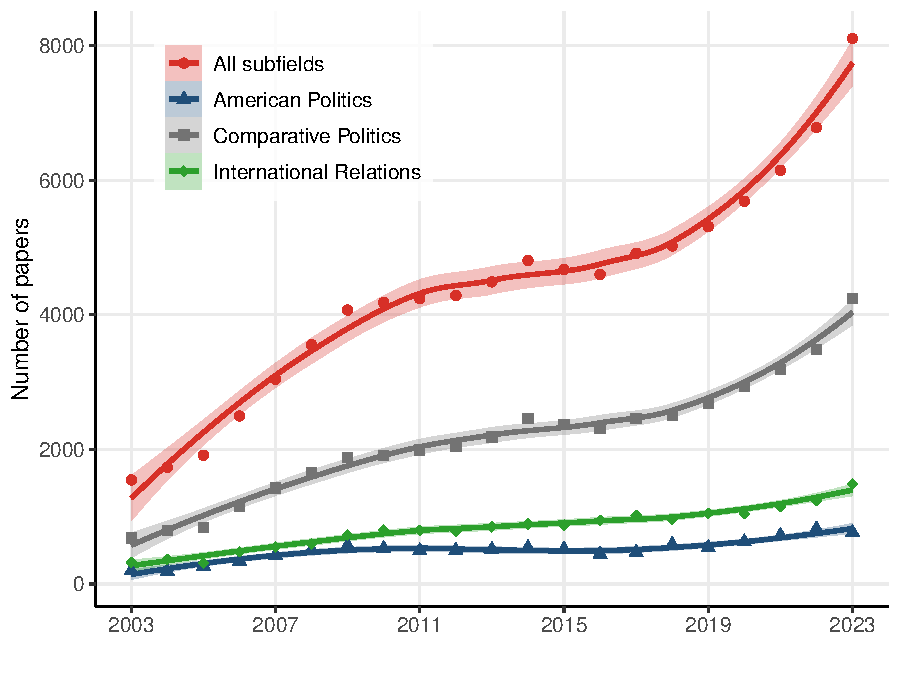
\includegraphics[width=0.7\textwidth, height=0.8\textheight, keepaspectratio]{Figures/fs0_trends.pdf}
    \vspace{-1em}
    \caption{Number of papers published each year in our full sample from 2003 to 2023 ($n=91,632$) and by subfield, with loess fits. The red line shows total papers; blue, American Politics; gray, Comparative Politics; and green, International Relations.}
    \label{fig:trends}
\end{figure}

Next, we obtained full-text versions of the articles where possible and successfully retrieved the complete text for 91,632 articles from 156 different journals. Full-text availability varies somewhat across publishers and subfields, so the full-text corpus is broad but not exhaustive. We then used a combination of supervised machine learning and a commercial LLM, \texttt{gpt-4o}, to classify complete-text articles along 19 research design dimensions (see description of the approach below). Figure~\ref{fig:trends} shows the yearly number of published papers in our full-text sample, both overall and by subfield. The volume of published political science work has grown rapidly. From 1,546 papers in 2003, the count has more than quadrupled to over 8,109 in 2023.\footnote{See \citet{grossman2025political} for an analysis of the factors underlying the dramatic increase in political science publication volume.}

\subsection*{Constructing Measures}

We construct a series of variables to characterize each paper's methodological features, substantive focus, and transparency practices. Details of the coding procedure appear in Section~\ref{sisec:prompt} in the Supplementary Materials. We first assign each paper a subfield label drawn from six categories: American Politics, Comparative Politics, International Relations, Methodology and Formal Theory, Political Theory and Philosophy, and Public Policy/Administration. The label reflects the paper's primary substantive contribution.

We then identify whether the paper is an \emph{empirical quantitative} study. A paper is coded as empirical quantitative if it conducts its own analysis of observational or experimental data, including reanalyses of existing datasets. Simulation exercises or purely methodological discussions without data are not included. Papers whose main method is qualitative, formal-theoretic, or normative are coded as non-quantitative for our purposes. We further assign one of three general goals---descriptive, explanatory, or predictive---only to empirical quantitative papers.

Explanatory papers investigate the causes or consequences of social phenomena and develop evidence consistent with one or more causal relationships, even if they do not always use explicit causal language. Descriptive papers center their contribution on measurement or characterization, for example by introducing new indicators, establishing baseline levels, or documenting group differences, without developing or testing a causal mechanism. Predictive studies focus on forecasting an outcome or identifying variables that best predict it, typically using out-of-sample or cross-validated performance as an evaluation criterion, and do not interpret those variables as causes. In cases where papers combine elements of these goals, we code the general goal based on the paper's primary contribution. Because causal claims are generally not used in predictive and descriptive work, we restrict our coding of primary research design to papers classified as explanatory. 


\begin{figure}[!ht]
    \centering\vspace{-1em}
    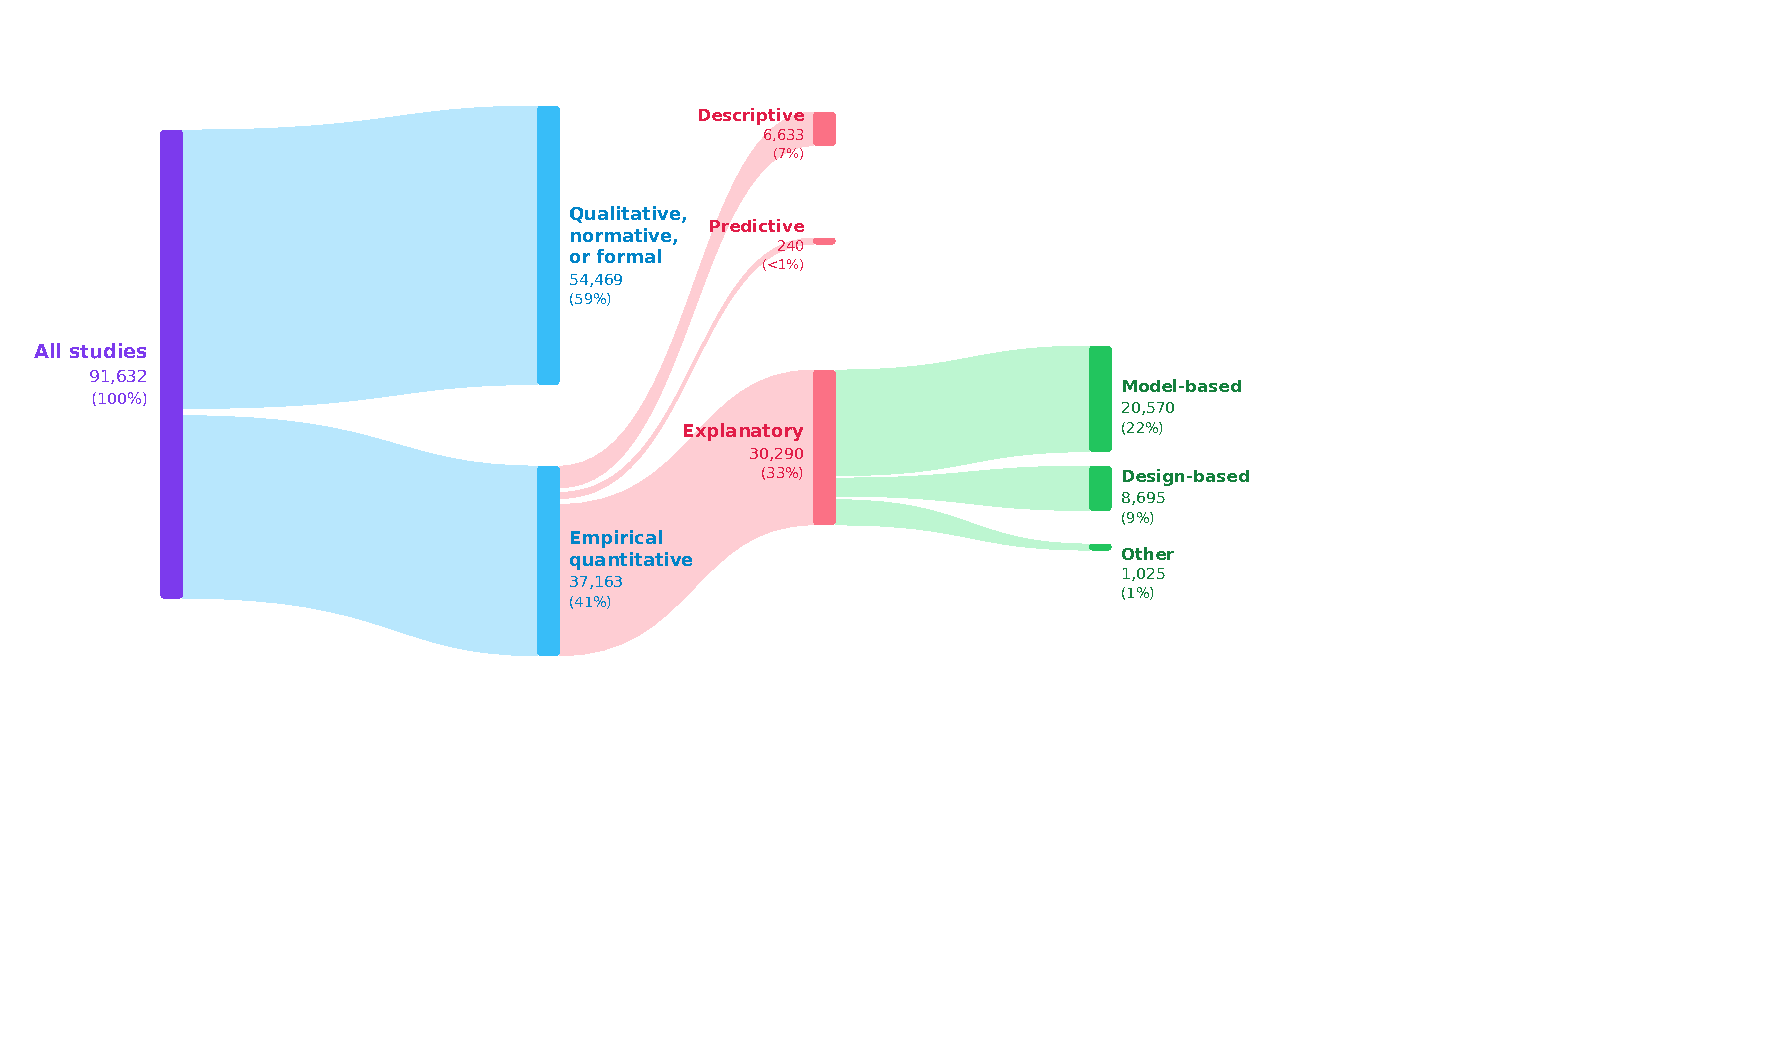
\includegraphics[width=1\linewidth]{Figures/sankey_diagram.pdf}\vspace{-3em}
    \caption{Sequential classification of type of studies. Flows trace papers from the full sample to quantitative studies, then to descriptive, predictive, and explanatory goals, and finally to design-based versus model-based and other approaches. The percentage numbers use the full sample of studies, $91,632$, as the denominator.
}
    \label{fig:sankey}
\end{figure}

Figure~\ref{fig:sankey} illustrates this sequential classification. We highlight two important patterns from our classification. First, quantitative, empirical papers are a minority, representing 41\% of all papers pooled across years. Second, within quantitative work, explanatory papers dominate (81\%). Descriptive papers constitute only 18\% of empirical quantitative papers. Predictive papers remain rare (240 across the entire period). Averages over two decades may mask important temporal dynamics. Figure~\ref{fig:quantemptime} shows that the share of empirical quantitative papers has increased steadily, reaching about 48\% by 2023. Disaggregation by subfield reveals similar upward trends but persistent differences in baseline levels: In 2023, 27\% of International Relations papers use quantitative methods, compared to 57\% in Comparative Politics and 84\% in American Politics.

\begin{figure}[!ht]
    \centering
    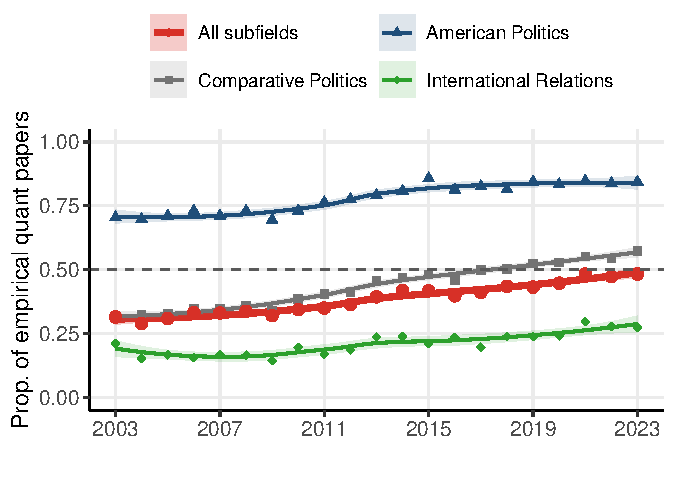
\includegraphics[width=0.7\textwidth, height=0.8\textheight, keepaspectratio]{Figures/fs1_empirical_overall_and_subfields.pdf}\vspace{-1.5em}
    \caption{The proportion of empirical quantitative papers overall and by subfield. The red curve shows the overall share, and the blue, gray, and green curves show trends for American Politics, Comparative Politics, and International Relations. Lines are lowess fits with 95\% confidence intervals; points indicate raw annual proportions.}
    \label{fig:quantemptime}
\end{figure}

For the $30,296$ explanatory empirical quantitative studies, which are the main focus of our analysis in the next section, we classify each paper's primary research design into three families: design-based, model-based, and other designs. {\it Design-based approaches} tie causal identification to a described source of exogenous or as-if-exogenous variation in treatment assignment (for example, randomized assignment, institutional cutoffs, policy shocks, or plausibly exogenous timing) and articulate the corresponding identification assumptions as claims about the assignment mechanism rather than as implications of the regression specification alone. Specifically, these approaches include experimental studies---field, survey, and lab experiments---and a range of non-experimental identification strategies based on unconfoundedness and overlap, such as matching and reweighting techniques; natural and quasi-experiments;\footnote{These studies use exogenous variation in treatment not controlled by the researcher, such as shocks or sudden institutional rules (e.g., natural disasters, draft lotteries, externally implemented policy changes). They fit within unconfoundedness designs, but researchers often analyze them with regression methods without explicitly stating unconfoundedness or selection-on-observables assumptions.} instrumental variable designs; regression discontinuity and regression kink designs; difference-in-differences designs;\footnote{This category includes broadly defined causal panel analysis under parallel trends \citep{chiu2023causal}. Its implementations include canonical difference-in-differences, two-way fixed effects models, event studies, longitudinal approaches to staggered treatment adoption, and related variants. All assume some version of the parallel trends assumption.} and the synthetic control method. Design-based methods account for 29\% of explanatory papers, suggesting substantial but still limited methodological transformation.

{\it Model-based approaches} support causal interpretation primarily through parametric or statistical modeling assumptions, including functional-form restrictions and conditional-independence claims embedded in the specification, and often operationalize causal questions via models such as linear regression, generalized linear models, structural equation models, and time-series models (for example, ARMA, GARCH, and vector autoregression). {\it Other methods} capture approaches not covered by these categories, including network analysis, text-as-data methods, agent-based modeling, and purely associational analyses such as bivariate correlations and crosstabs. 

Because linear regression can recover causal effects in both experimental and non-experimental settings \citep{angrist2009mostly, aronow2016does, imbens2025comparing}, we do not take the use linear regression as diagnostic of model-based research. Only studies that interpret coefficients from covariate-adjusted regressions as causal effects without a stated assignment mechanism or design-based identification argument are coded as model-based. In our corpus, 71\%, rely on simple regression analysis of this form.

For explanatory studies, we also code whether the paper states key identification assumptions, defined as explicit statements of the core assumption underlying the design (e.g., unconfoundedness, parallel trends, continuity, or exclusion restrictions). We also code whether quantitative explanatory papers make a causal claim. Explicit claims use terms such as ``causes,'' ``effect,'' or ``impact.'' Implicit claims are coded when the paper frames its contribution in terms of causes and consequences or interprets coefficients as causal, even if it avoids direct causal terminology. Initially, we also aimed to assess whether an explanatory study clearly articulated an interpretable estimand. However, consistent with \citet{lundberg2021your}, our pilot study indicated that, aside from papers employing experimental, IV, and RD designs—which typically target average treatment effects (ATE), average treatment effects on the treated (ATT), or local average treatment effects (LATE)---very few studies do so. Consequently, we dropped this measure.



We additionally code several features of the analysis, including sample size and the adoption of research practices intended to enhance credibility. These practices include: (1) whether the paper reports placebo tests, (2) whether it indicates that a power analysis was conducted, and (3) whether the hypotheses or the analysis were pre-registered. We focus on these three because they are commonly used across designs and are intended to reduce different forms of inferential error. Placebo tests and pre-analysis plans help reduce the risk of false positives, respectively by detecting spurious results~\citep{eggers2024placebo} and by limiting undisclosed analytic flexibility, i.e., p-hacking~\citep{, brodeur2024preregistration}. Power analyses reduce the likelihood of false negatives by ensuring adequate statistical power to detect meaningful effects, a concern that has grown salient in social science research \citep{arelBundock2026underpowered,lal2024much}. Although increasing sample size is not a research practice per se, we treat it as an indirect indicator of false negative sensitivity: if researchers are more attentive to power, they may design studies with larger samples regardless of whether they conduct formal calculations. Together, these measures allow us to document methodological choices, and causal reasoning across the quantitative political science literature.

Two caveats are in order. First, we measure these variables by taking what is reported in papers at face value. We do not assess how well authors executed a particular research design, whether the identifying assumptions they invoke are warranted in the application or not, or whether the paper contains errors or misrepresentations of methods. Second, our taxonomy is descriptive rather than evaluative or normative: it is not intended to encode any ranking in which design-based studies are treated as inherently more or less credible than model-based studies. For any given paper, the assumptions required for identification in either family can hold or fail in practice. Indeed, recent replication studies of political science research suggest that, across designs, problems with assumption validity, statistical power, and execution errors remain present \citep[e.g.,][]{stommes2023reliability, lal2024much, chiu2025causal}.

\subsection*{LLM pipeline and human validation.}

We next describe how we coded them at scale. We developed an LLM-based coding framework and conducted a structured human validation to generate reliable measures from our corpus of political science articles. We first gathered the raw text of all scraped papers and truncated any article exceeding 50,000 tokens (about 35,000 words) to manage cost and ensure processing efficiency. In practice, this affected only a small number of long review articles, and truncation typically removed appendices rather than main empirical content. We then sent each paper's text, together with a custom prompt, to OpenAI's \texttt{gpt-4o} model via the batch API. The System Prompt outlined 19 research dimensions to code, including research design, transparency practices, and causal claims (see Supplementary Materials). Using OpenAI's structured outputs, we constructed a \texttt{JSON} schema to ensure consistent formatting, and the model coded each article according to this schema. To refine the prompt, we iteratively tested eight versions by qualitatively evaluating outputs for a sample of 116 papers. Each author read a couple dozen papers, noted errors, and proposed revisions. After eight rounds, we finalized the prompt and evaluated it on the five key variables.

We validated five core variables with human coders that anchor our main analysis: (1) whether a paper is an empirical quantitative study, (2) its subfield, (3) its primary research design, (4) whether it states key identification assumptions, and (5) whether it makes a causal claim. Subfield and research design are multi-label variables spanning six and seventeen categories; the remaining variables are binary. Task~1 evaluated whether papers were empirical and quantitative using a random sample of 200 papers. Task~2 assessed the remaining variables using another 200 papers identified by the model as empirical and quantitative, with one paper removed after review. Four research assistants coded each paper in pairs, with disagreements resolved by a third coder in consultation with an author. Although modest relative to the corpus, these samples are sufficient to estimate accuracy with useful precision, and additional spot checks across journals yielded similar patterns. Accuracy was high: Task~1 reached 98\% agreement with human coders. In Task~2, accuracy was 83\% for subfield, 73\% for research design (84\% among design-based studies), 78\% for identification assumptions (90\% among design-based studies), and 82\% for causal claims (87\% among design-based studies). See section \ref{sisec:prompt_validation} for more details.
% Errors were concentrated in three areas, each occurring only occasionally: (a) misclassifying theoretical or methodological work, (b) collapsing quasi-experiments into generic labels, and (c) overlooking random assignment in experiments.

Overall, these exercises show that LLMs can generate reliable large-scale measures of methodological features in political science when supported by targeted human checks. The LLM performs notably better among design-based studies because these papers tend to have more structured methods sections, which affects coding difficulty. 


\section*{Main Findings}

To evaluate how quantitative empirical research in political science has changed as a consequence of the credibility movement, we present descriptive evidence on the scope and pace of methodological change across the discipline. We examine shifts in research designs, empirical practices, and differences in scholarly reward between studies adopting design-based methods and those using traditional approaches.

\paragraph*{Design-Based Methods Rose Steadily But Unevenly}

How have methodological practices shifted in quantitative explanatory research? If the credibility revolution has taken hold, design-based strategies should increasingly displace model-based approaches. Figure~\ref{fig:basictrends}(a) traces these aggregate trends from 2003 to 2023. Model-based methods (gray) dominated for most of the period, but design-based approaches (black) rose from 15\% to 40\%. By 2023, the two approaches accounted for nearly equal shares of explanatory quantitative research, while other methods, a residual category defined above, constitute 18\%. 
\begin{figure}[!ht]
    \centering
    \begin{subfigure}[b]{0.47\textwidth}
        \centering
        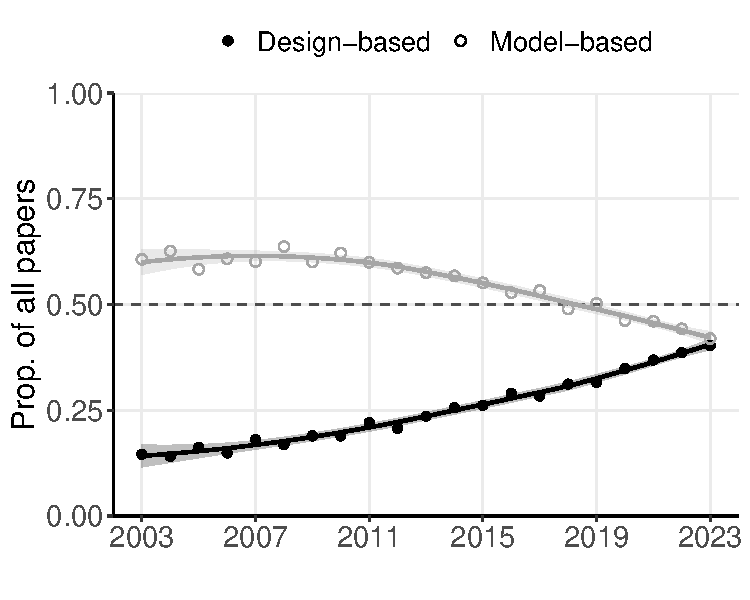
\includegraphics[width=\linewidth]{Figures/qe_design_overall.pdf}
        \caption{Design-based vs. model-based studies}
        \label{fig:design_overall}
    \end{subfigure}    \hfill
    \begin{subfigure}[b]{0.47\textwidth}
        \centering
        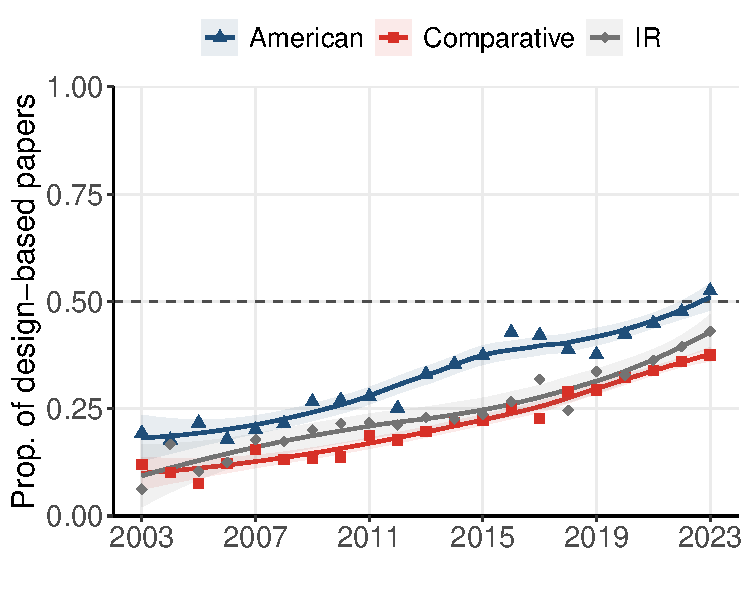
\includegraphics[width=\linewidth]{Figures/qe_design_subfields_shapes.pdf}
        \caption{Design-based studies by subfield}
        \label{fig:design_subfields}
    \end{subfigure}

    \caption{Trends in the use of design-based methods among explanatory empirical quantitative papers.}
    \label{fig:basictrends}
\end{figure}
Within this overall shift, subfield differences are relatively modest. As Figure~\ref{fig:basictrends}(b) shows, American Politics was an earlier adopter of design-based approaches, but by 2023 all three major subfields show substantial adoption: American Politics at 52\%, International Relations at 43\%, and Comparative Politics at 38\%. 

Figure~\ref{fig:basictrends_nosurvey}(a) in the Supplementary Materials  reports overall results excluding survey experiments. Within this subset, the proportion of design-based papers is considerably smaller: 12\% of quantitative papers in 2003, rising to 27\% in 2023. Conversely, model-based methods remain dominant throughout, accounting for more than half of all quantitative papers in 2023. Figure~\ref{fig:basictrends_nosurvey}(b) in the Supplementary Materials shows the subfield specific trends when excluding survey experiment. This exclusion reduces the share of design-based papers most starkly for American Politics. Specifically, the difference is of 21 percentage points (pp) in 2023, relative to the proportion when survey experiments are included. Conversely, the difference is slightly smaller for IR in 2023, a 14.5 pp difference that same year and smallest for Comparative Politics with a reduction of only 10.5 pp that year.

%To further understand which specific designs drive this growth, Figure~\ref{fig:designshare} breaks down the composition of design-based work. As expected from the results reported in Figure~\ref{fig:basictrends_nosurvey}(a) survey experiments account for much of the increase in design-based methods and become the single most common design by 2023. Difference-in-differences and matching or reweighting methods based on unconfoundedness also expand, while instrumental variables, field experiments, and regression discontinuity designs maintain smaller but steady shares. Natural/quasi-experiments and synthetic control remain rare.

Next, we examine which specific designs drive this growth and how each method has evolved over time. Figure~\ref{fig:bymethods2} traces these trajectories for both experimental and non-experimental approaches. Figure~\ref{fig:bymethods2}(a) reports trends for the three experimental approaches. Survey experiments, which account for much of the increase in design-based methods, grow rapidly, rising from about 4\% of all explanatory quantitative studies in 2003 to more than 15\% by 2023, and constitute roughly 45\% of all design-based research by the end of the period. Field experiments remain uncommon, arguably due to their high cost, but show a modest upward trend. By contrast, lab experiments decline sharply after 2016. This decline likely reflects the increasing availability of online and survey-based experimental platforms, which allow researchers to conduct experiments at lower cost, with larger and more diverse samples, and without the logistical constraints of in-person laboratory settings.

%\begin{figure}[!ht]
 %   \centering
  %  \includegraphics[width=0.9\linewidth]{Figures/qrd1_area_v2.pdf}
   % \caption{Relative share of design-based studies in all explanatory empirical quantitative studies, by year.}
    %\label{fig:designshare}
%\end{figure}

Figure~\ref{fig:bymethods2}(b) reports trends for six non-experimental design-based methods. Difference-in-differences (including its various implementations) grows almost monotonically and reaches more than 6\% of all explanatory empirical quantitative papers in 2023. Matching and reweighting methods increased to about 5\% around 2012 before plateauing through the end of the period. Instrumental variable designs rose from 3\% in 2003 to nearly 5\% in 2012, then gradually declined over the past decade. Regression discontinuity designs increase slowly but remain near 2\% in 2023, reflecting limited opportunities for such designs. Natural and quasi-experiments remain around 1\% of explanatory empirical quantitative studies throughout. Synthetic control methods appeared around 2012 and have increased modestly in recent years, but still constitutes less than 1\% of explanatory empirical quantitative papers.

Taken together, these patterns show that the credibility revolution has altered methodological practice, but unevenly across designs. Survey experiments, to the extent that they can be conceptualized as design-based methods, account for most of the overall shift, followed by difference-in-differences designs, while other design-based approaches have grown only modestly or remained niche.

\begin{figure}[!ht]
    \centering

    \begin{subfigure}[b]{0.9\textwidth}
        \centering
        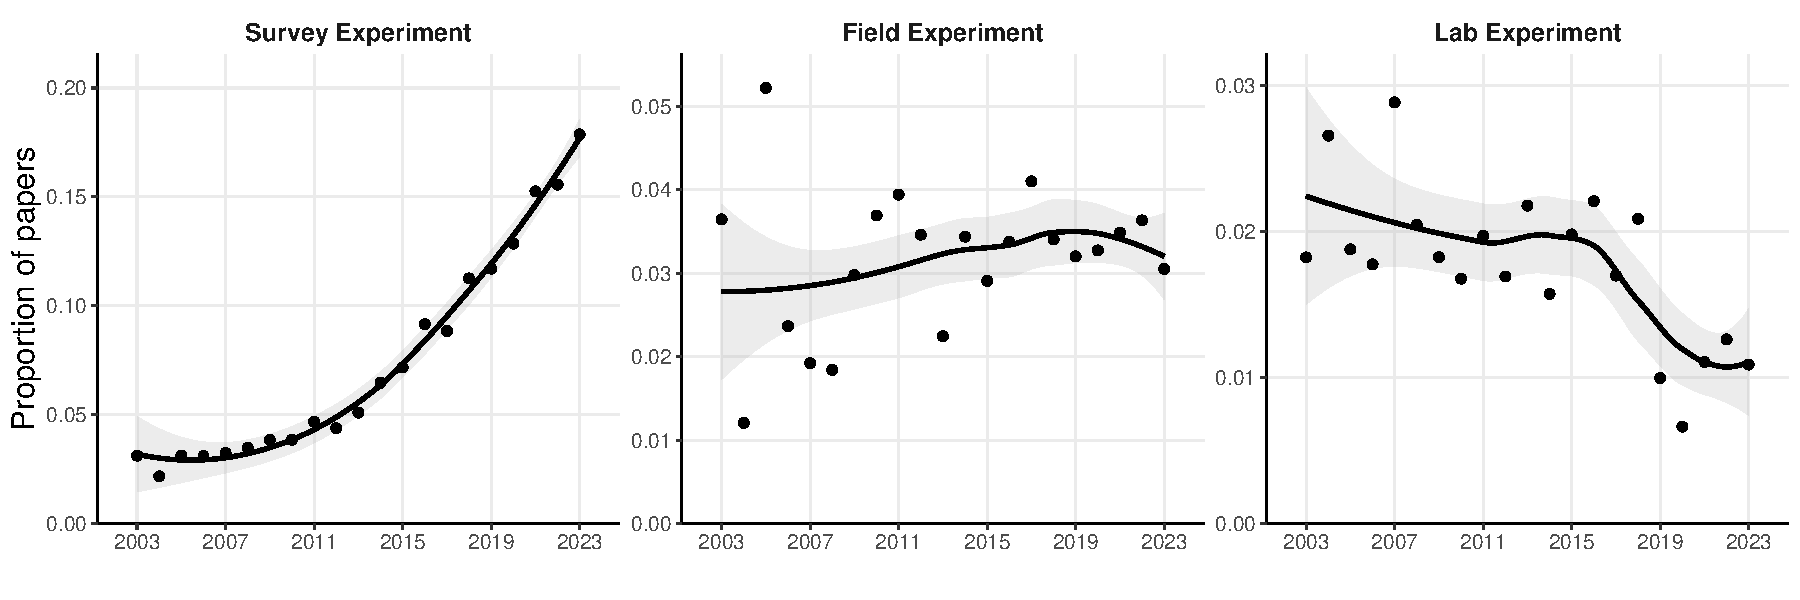
\includegraphics[width=\linewidth]{Figures/qrd2_lines_rd_experiment.pdf}
        \caption{Experimental}
        \label{fig:design_overall}
    \end{subfigure}
    \hfill
    \begin{subfigure}[b]{0.9\textwidth}
        \centering
        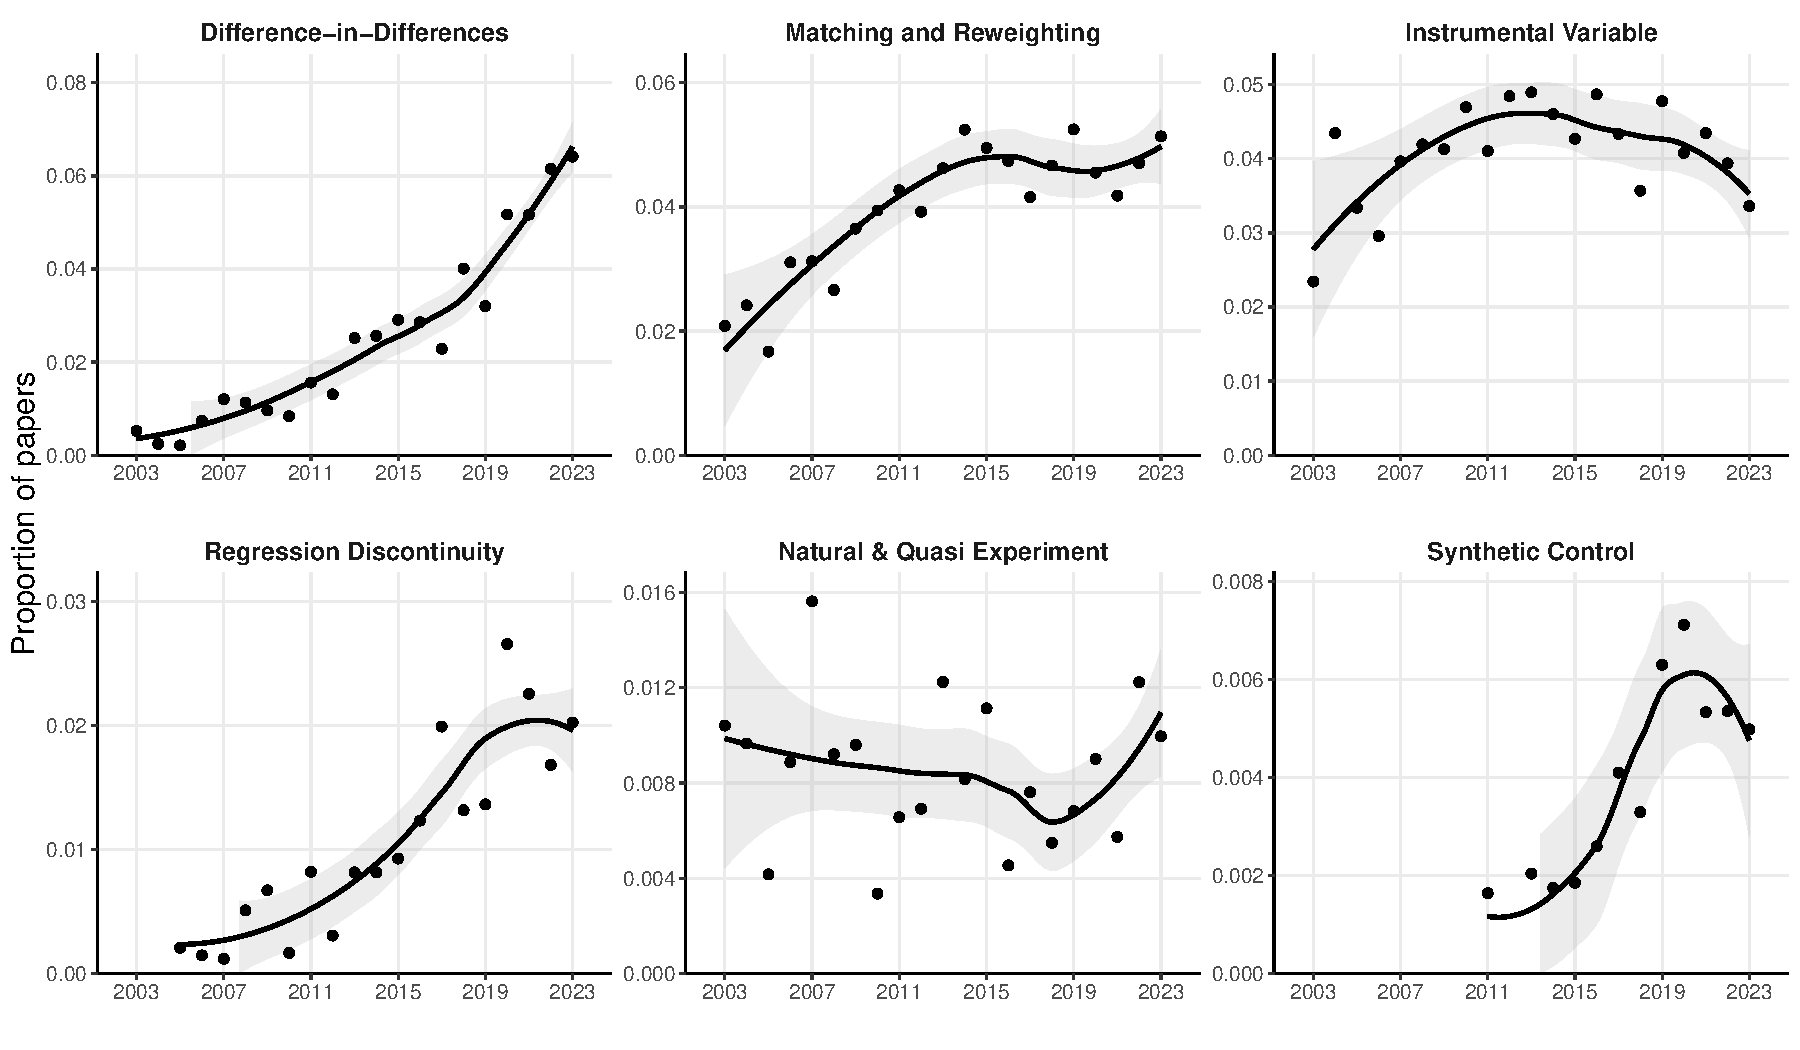
\includegraphics[width=\linewidth]{Figures/qrd2_lines_rd_rest.pdf}
        \caption{Non-experimental}
        \label{fig:design_subfields}
    \end{subfigure}

    \caption{Popularity of design-based methods by year. The denominator is the total number of explanatory empirical quantitative studies in each year.}
    \label{fig:bymethods2}
\end{figure}

%\FloatBarrier

\paragraph*{Design-based studies are concentrated in influential journals.} We found that design-based methods have risen slowly but steadily over the last two decades, reaching parity with traditional model-based approaches in 2023. This pattern suggests that credibility-revolution practices have diffused at a modest pace and remain far from universal. One concern, however, is that treating all articles equally may mask differences across publishing venues. More influential journals may adopt emerging methodological standards earlier and thereby shape broader disciplinary expectations. If so, equal weighting could understate both the extent and the speed of change occurring in more widely read higher-impact outlets.

\begin{figure}[!ht]
    \centering

    \begin{subfigure}[b]{0.47\textwidth}
        \centering
        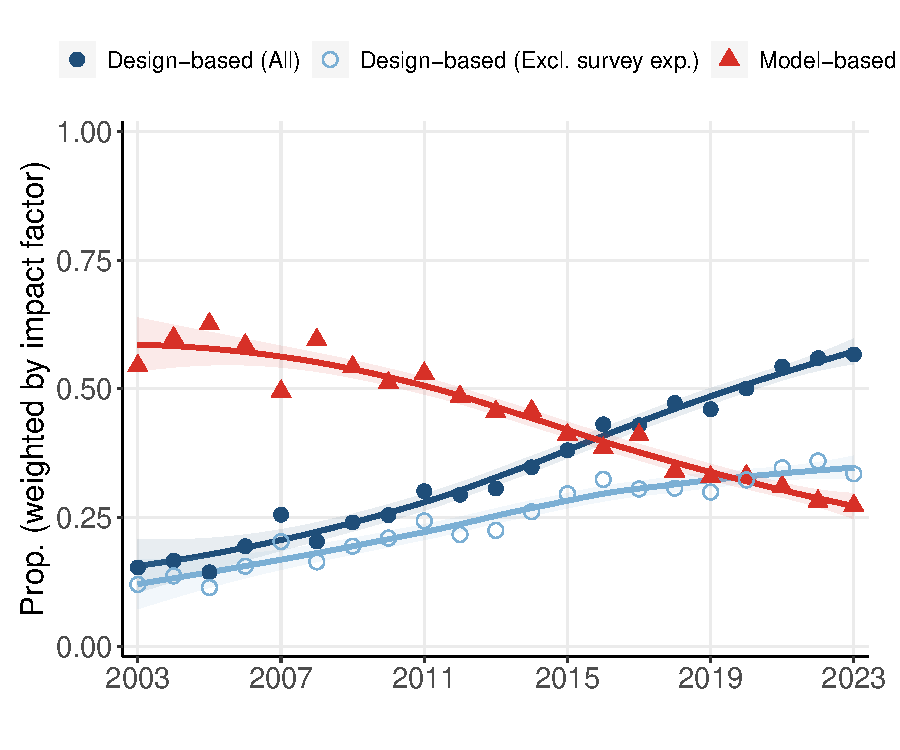
\includegraphics[width=\linewidth]{Figures/qe_basic_trends_weighted_top20_surveycomp.pdf}
        \caption{Studies published in top 20 journals}
        \label{fig:top20weighted}
    \end{subfigure}
    \hfill
    \begin{subfigure}[b]{0.47\textwidth}
        \centering
        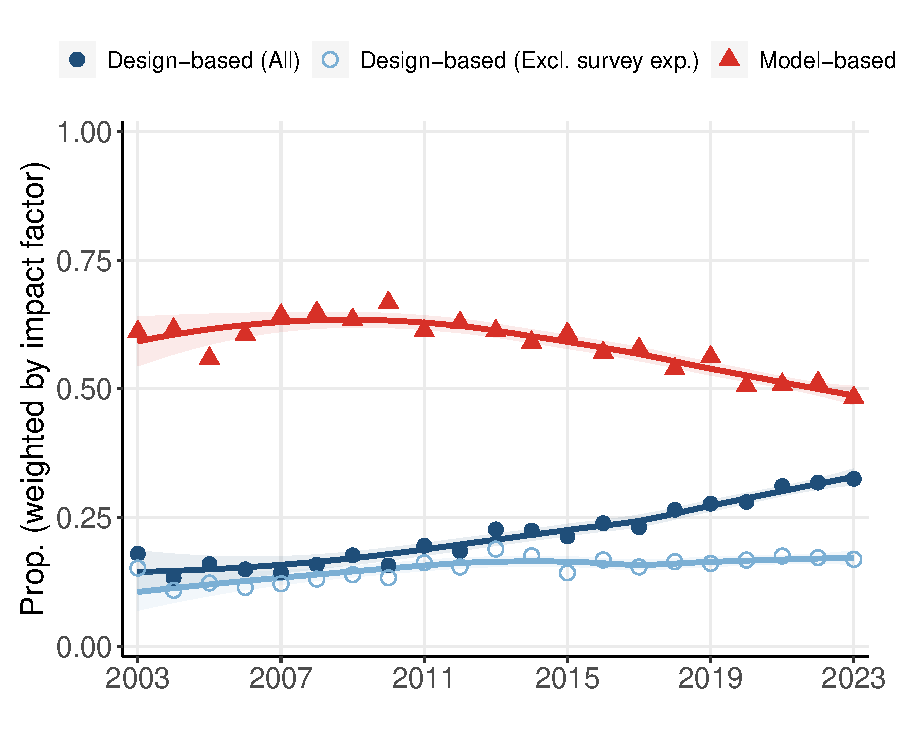
\includegraphics[width=\linewidth]{Figures/qe_basic_trends_weighted_nottop20_surveycomp.pdf}
        \caption{Studies published in other journals}
        \label{fig:bottomrest}
    \end{subfigure}
\caption{Proportion of design-based and model-based studies by journal ranking, including and excluding survey experiments from the sample. The denominator is the total number of explanatory empirical quantitative studies published each year, weighted by SJR (a measure of journal impact). Observations are weighted by SJR. The left panel shows papers in the top 20 journals; the right panel shows papers in other journals. Curves with 95\% confidence intervals are lowess fits.}
    \label{fig:weighted}
\end{figure}

To assess this possibility, Figure~\ref{fig:weighted} plots the share of design- and model-based studies among explanatory quantitative articles, weighting each article by the SJR score of its publishing journal. The left panel reports trends for the 20 highest-impact journals; the right panel reports all remaining outlets. Darker shades include survey experiments, while lighter shades exclude them. After weighting, design-based approaches rise more rapidly in the highest-impact journals. The weighted proportion of design-based papers eventually surpasses that of model-based work, although the timing of this crossover depends on whether survey experiments are included. When survey experiments are included in the category, design-based work overtakes model-based work in 2016; when they are excluded from the numerator, the crossover occurs in 2021. In contrast, model-based approaches remain predominant in lower-impact outlets throughout the period, despite a gradual increase in design-based research. Excluding survey experiments almost completely flattens this increase, indicating that survey experiments account for a large share of design-based output in the discipline overall, even after adjusting for journal impact. Taken together, these patterns show that methodological change has been concentrated in the most visible and influential segment of the discipline. 

Impact-factor weighting adjusts for differential influence across papers but does not reveal where those differences originate. Figure~\ref{fig:journals} shows the proportion of design-based studies among the top 20 political science journals between 2019 and 2023, and estimates that include survey experiments (circles) from those that exclude them (triangles). A first takeaway is that there is substantial heterogeneity within the top-20 journals, with some publishing relatively low proportions and some publishing comparatively high proportions of design-based studies.\footnote{\emph{Political Analysis} publishes a substantially lower proportion of design-based studies than other top 10 journals, reflecting its role as a methods journal, which prioritizes the development of statistical and computational approaches over the application of design-based designs to substantive empirical questions.} While the share of design-based research exceeds 55\% of papers published in \emph{Quarterly Journal of Political Science} and \emph{Political Science Research and Methods} in other top-20 journals, such as {\it Journal of European Public Policy} and {\it European Union Politics}, this share is below 20\%. 

\begin{figure}[!ht]
    \centering
    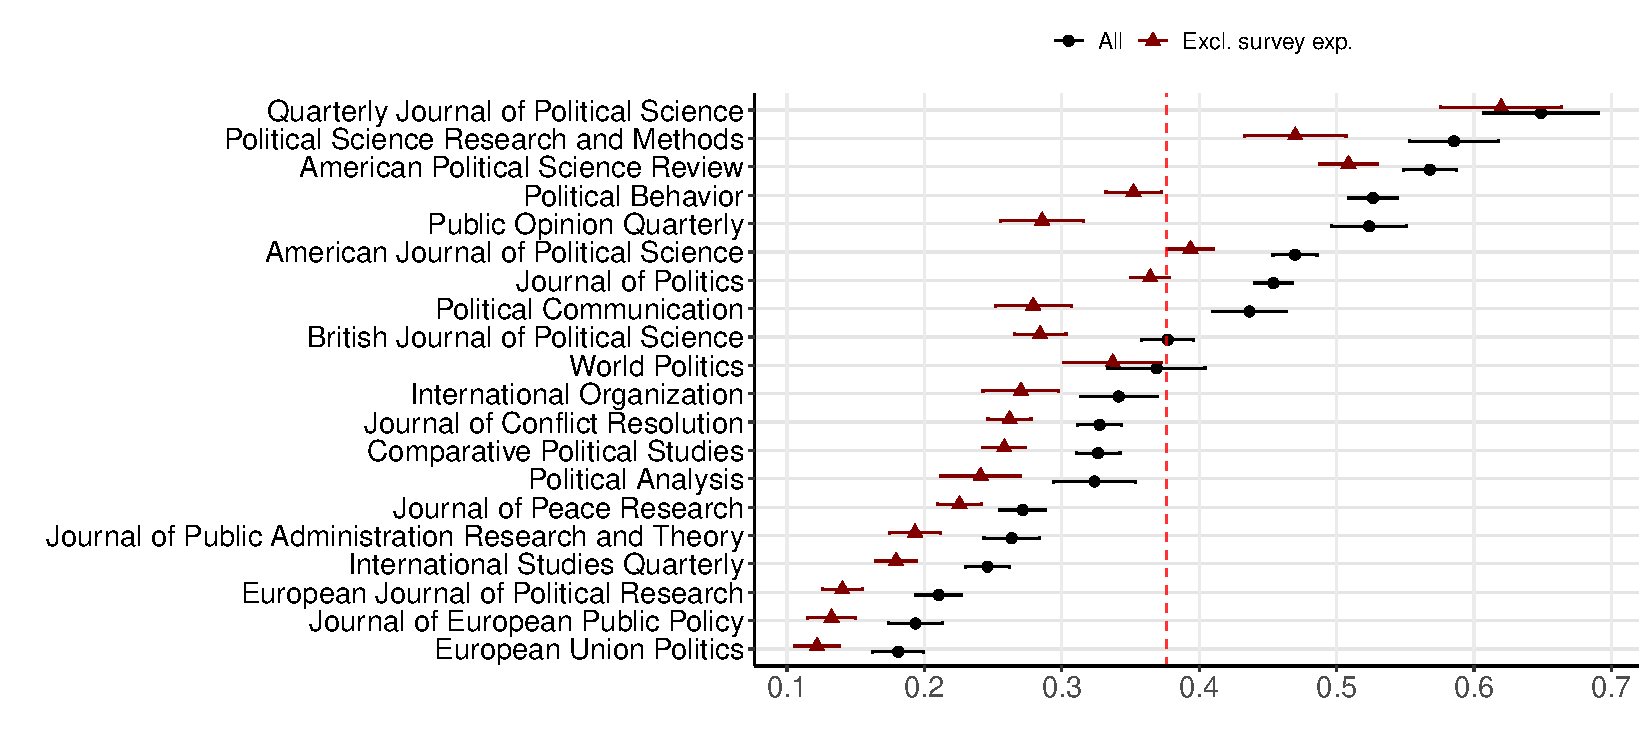
\includegraphics[width=1\linewidth]{Figures/qrd5_credible_byjournal_rd_surveys_top20.pdf}
    \caption{Proportion of design-based studies among top-20 political science journals (by SJR score) with 95\% confidence intervals. The numerator is the number of design-based studies published between 2003 and 2023. The denominator is the total number of explanatory empirical quantitative papers published during the same period. Journals ranked as top-10 by SJR are painted in black. Circles represent proportions including survey experiments in design-based studies and triangles represent proportions excluding survey experiments. }
    \label{fig:journals}
\end{figure}

A second noticeable pattern concerns the heterogeneity in the gap between the journal-specific estimates that include and exclude survey experiments in the proportion of design-based research. Some outlets have large gaps, others smaller gaps. For instance, large gaps in opinion-focused journals such as \emph{Public Opinion Quarterly} and \emph{Political Behavior} are consistent with the origins of survey experiments in social psychology and survey research. More surprising are the gaps observed in general-interest journals. For instance, in the \emph{American Political Science Review}, the share of design-based work falls from 57\% to 51\% when survey experiments are excluded, with similar patterns in the \emph{American Journal of Political Science} (47\% to 39\%) and in the \emph{Journal of Politics} (45\% to 36\%). Although these estimates pool all paper-years, these gaps indicate that survey experiments have become an important method in general-interest outlets, not only in substantively opinion-focused venues.

\FloatBarrier

\paragraph*{Authors from higher-ranked institutions are more likely to adopt design-based methods.} Results thus far show that design-based methods were adopted earlier---and are more common--in high-impact influential journals than in other outlets. This pattern raises the possibility of uneven diffusion across the discipline. To explore this, we examine authors' institutional affiliations as an additional indicator. Institutional rank offers a complementary perspective on whether uptake has varied across different segments of the discipline.

We use the Shanghai Academic Ranking of World Universities (ARWU) to rank institutions. We extracted institutional affiliations for all authors and matched 77,123 author–institution pairs to Shanghai-ranked universities across 59,248 papers, covering 65\% of our full-text sample. For each paper, we compute the average rank of the authors’ institutions. Details on the matching procedure appear in the Supplementary Materials.

Figure~\ref{fig:institutional} shows the adoption of design-based methods by authors’ institutional rank, again reporting estimates that include survey experiments (black) and exclude them (red). Among authors affiliated with the top 40 institutions, adoption rates decline gradually with rank. At the very top of the distribution, design-based approaches account for roughly 50\% of studies in the full corpus and about 40\% when survey experiments are excluded. These shares fall steadily to approximately 28\% when survey experiments are included and about 20\% when they are excluded by rank~40, after which adoption rates level off for lower-ranked institutions. The persistence of this gradient when survey experiments are excluded indicates that the association between institutional rank and design-based adoption is not driven solely by survey experiment use. Instead, these patterns suggest that the methodological shift associated with the credibility revolution has been more pronounced among authors at highly ranked institutions, extending beyond any single design-based method.

\begin{figure}[!ht]
    \centering\vspace{-0.5em}
    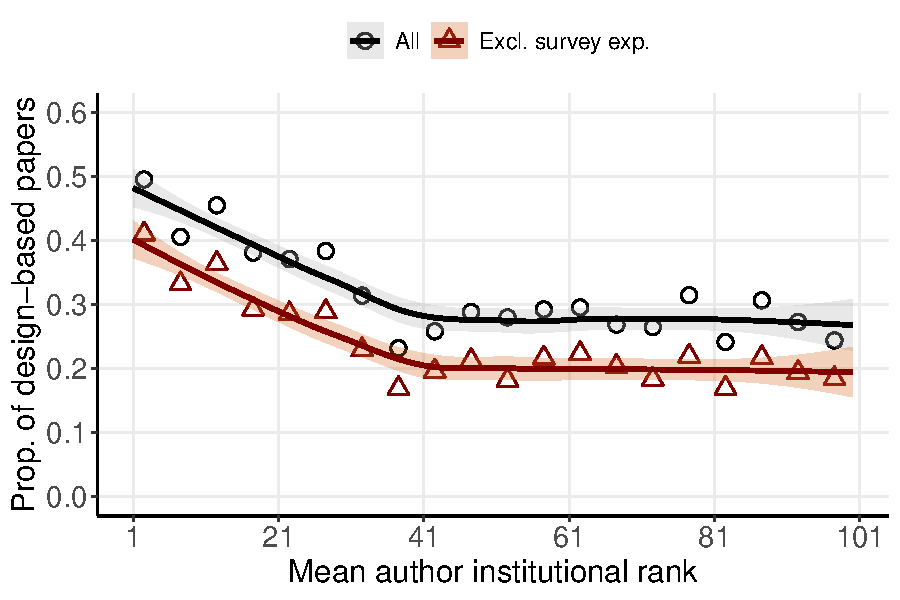
\includegraphics[width=.7\linewidth]{Figures/qe_institutionl_top100_comparison.pdf}
    \caption{Adoption of design-based methods by authors' average institutional rank, including and excluding survey experiments from the sample. The denominator is the total number of explanatory empirical quantitative studies at each ventile ($1/20$). Lower ranks indicate more prestigious institutions. The sample includes all papers with institutional affiliation data matched to Shanghai rankings. Circles represent means of 20 bins, and the lines show lowess curves with 95\% confidence intervals.}
    \label{fig:institutional}
\end{figure}

This concentration parallels the journal-tier patterns. Whether it reflects early uptake that will diffuse more widely or a more persistent stratification remains uncertain. What is clear is that even among scholars in highly ranked institutions, the shift has been gradual: design-based methods took nearly two decades to reach parity with model-based approaches. Moreover, within design-based work, the rise has been driven primarily by survey experiments rather than broad adoption across multiple design-based strategies.

\paragraph*{Credibility-enhancing practices progressed modestly.}\label{errorates}

Beyond research design, scholars may adopt research practices aimed at mitigating inferential risks and bolstering the credibility of explanatory claims. We organize these practices along two dimensions: those oriented toward reducing false positive findings and those aimed at reducing false negative findings. We examine four indicators: the use of placebo tests and pre-analysis plans, which are commonly intended to limit false positives, and sample size and power analysis, which are commonly intended to reduce the likelihood of false negatives. We report trends separately for experiments, design-based observational studies, and model-based studies, since expectations and norms differ across designs and pooling would obscure meaningful distinctions.

Figure~\ref{fig:errorates} presents the results. Practices that mitigate false positives have expanded primarily within design-based research, but with notable variation across experimental and non-experimental work. Placebo tests remain concentrated in design-based observational studies, increasing from under 5\% in 2003 to around 20\% in 2023. Pre-analysis plans, by contrast, are concentrated in experimental research, appearing in roughly 35\% of such papers by 2023. They remain rare in design-based observational studies (about 3\%) and nearly absent in model-based work (under 1\%).

Practices oriented toward reducing the risk of false negatives show broader adoption. Most notably, median sample sizes increased substantially across all research designs between 2003 and 2023: from 490 to 1,601 in experiments, 984 to 2,059 in model-based studies, and 784 to 3,019 in design-based observational work. This trend is consistent with growing attention to statistical power, even in the absence of formal calculations. At the same time, sample size is a noisy indicator of such attention. Increases may reflect mechanical features of data accumulation over time, such as longer panel series, as well as shifts in empirical focus from national to subnational units of analysis that mechanically generate more observations.
 Power analyses themselves remain largely limited to experimental work, rising from 4\% to about 15\% between 2003 and 2023. They remain rare in design-based observational (under 2\%) and model-based research (0.6\%), despite their potential relevance for interpreting null findings across designs. These latter findings are consistent with recent research documenting low statistical power in published social science articles \citep{arelBundock2026underpowered}.


\begin{figure}[!ht]
    \centering

    \begin{subfigure}[b]{0.9\textwidth}
        \centering
        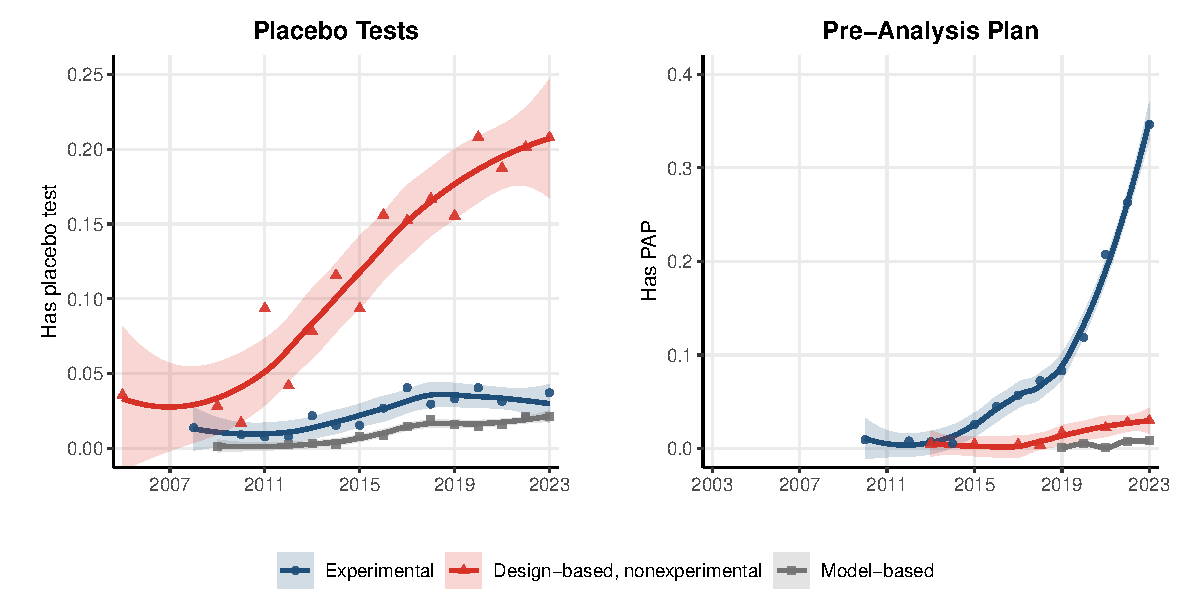
\includegraphics[width=\linewidth]{Figures/qe_type1_errors.pdf}
        \caption{False positive inference}
        \label{fig:type1}
    \end{subfigure}
    \hfill
    \begin{subfigure}[b]{0.9\textwidth}
        \centering
        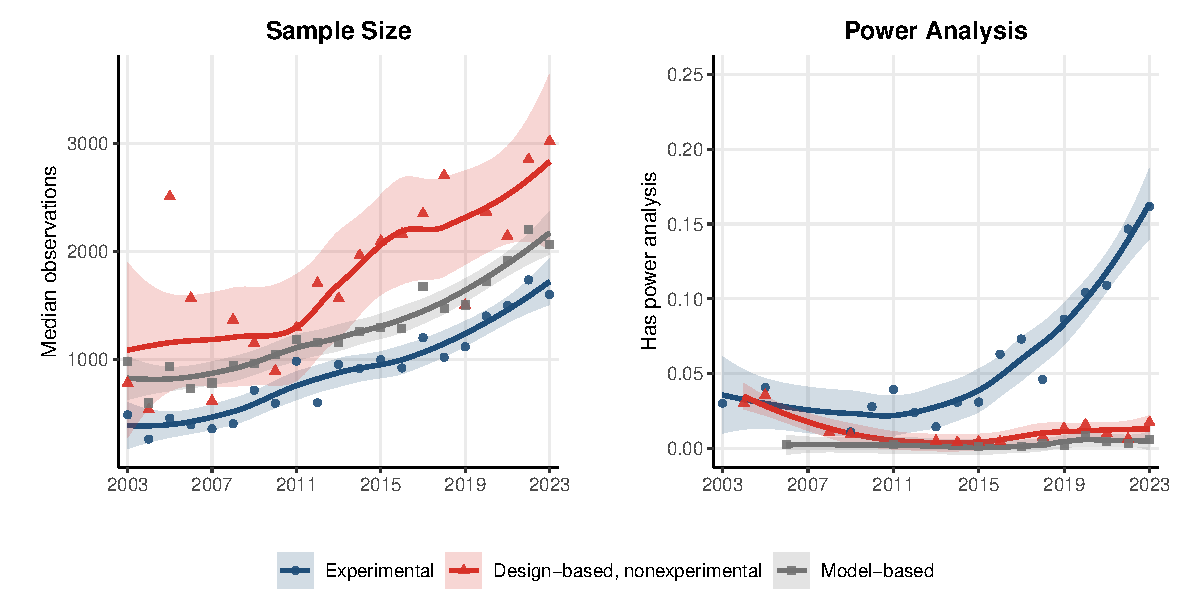
\includegraphics[width=\linewidth]{Figures/qe_type2_errors.pdf}
        \caption{False negative inference}
        \label{fig:top2}
    \end{subfigure}
\caption{Methodological practices by research design type. Panel (a) shows practices that reduce false positives: placebo tests and pre-analysis plans. Panel (b) shows practices that reduce false negatives: sample size and power analysis.}\label{fig:errorates}
\end{figure}

Taken together, these patterns indicate a gradual—but uneven—diffusion of practices aimed at reducing both false positive and false negative findings. Practices intended to limit false positives have expanded primarily within design-based research, with experimental and observational studies adopting different tools and with little uptake in model-based work. Practices that can reduce the likelihood of false negatives show broader reach: sample sizes have increased substantially across all research designs, including model-based studies, even as formal power analysis remains largely confined to experimental research. Nonetheless, adoption remains limited in absolute terms. Even within design-based research, none of these practices has become routine.



\iffalse

\subsection*{Credibility-Enhancing Practices Progressed Modestly}\label{sec:notgood} 

Research design is not the only source of credibility in quantitative causal inference. Scholars also rely on empirical practices that strengthen the plausibility of their claims. Pre-analysis plans, for instance, constrain researcher discretion and reduce the risk of $p$-hacking. Original survey data collection enhances credibility by enabling precise measurement of key variables and confounders, minimizing measurement error and omitted variable bias. Placebo tests further demonstrate that identifying variation operates through the theorized mechanism rather than spurious channels. Power analyses similarly bolster credibility by assessing whether a study is adequately equipped to detect meaningful effects, thereby reducing the likelihood of Type~II errors and clarifying the evidentiary value of null findings. Importantly, these credibility-enhancing tools often complement but are not limited to design-based approaches: researchers using model-based methods can, for example, employ placebo tests (e.g., showing that treatment does not affect prior outcomes) or use simulations to assess statistical power.

We examine six dimensions of empirical practice used to enhance the credibility of causal claims: (1) sample size, (3) original survey data collection; (3) placebo tests,
(4) explicit statement of identification assumptions, (5) pre-analysis plans, and (6) power analysis.\footnote{We also explored other criteria, such as clearly stating the causal quantity of interest, but we found it is highly correlated with the adoption of design-based methods. In other words, it is very rare to see researchers using model-based methods to define such quantities explicitly.} We assess the prevalence of these practices separately for experiments, design-based observational studies, and model-based approaches. This disaggregation reflects the fact that disciplinary norms impose some credibility practices more strongly on experiments than on observational research, and pooling them would obscure meaningful differences in trends.

Figure~\ref{fig:goodsigns} reports results for sample sizes, original data collection, placebo tests, and explicit statements of identification assumptions. Sample sizes increased substantially across all three categories. Experiments had median sample sizes of 490 in 2003, growing to 1,601 by 2023. The number of observations in studies with model-based methods grew from 984 in 2003 to 2,059 by 2023. For design-based observational studies, the number started at 784 in 2003 and reached 3,019 by 2023, showing the steepest growth. All else equal, these increases imply better-powered research regardless of method.

\begin{figure}[!ht]
    \centering\vspace{-1em}
    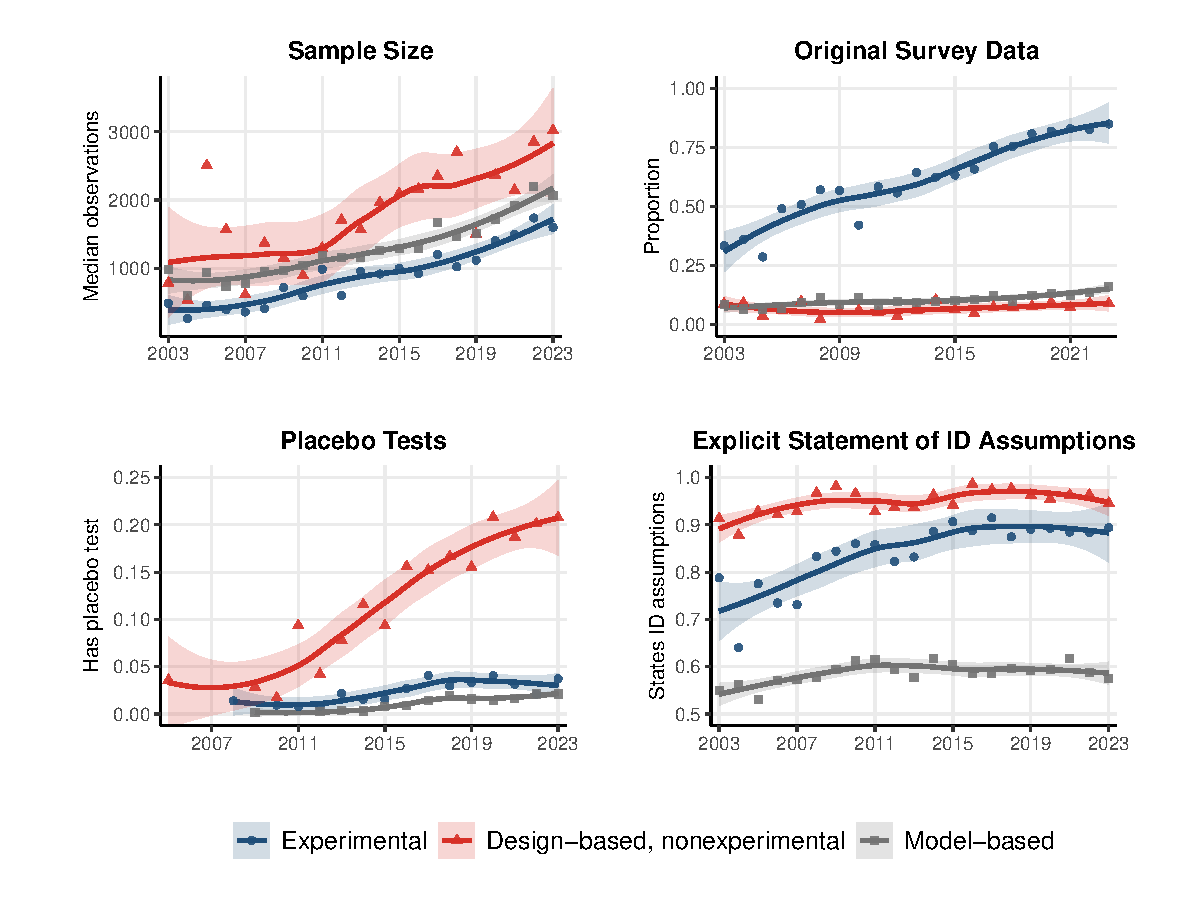
\includegraphics[width=1\linewidth]{Figures/qe_good_signs.pdf}
    \vspace{-2.5em}
    \caption{Transparency and credibility practices over time for quantitative explanatory papers. Top left: median sample size. Top right: proportion using original survey data. Bottom left: proportion conducting placebo tests. Bottom right: proportion explicitly stating identification assumptions. Experimental, design-based nonexperimental, and model-based studies are in blue, red, and gray, respectively.}
    \label{fig:goodsigns}
\end{figure}

As expected, experimental research relies heavily on original data collection, with nearly 75\% of experimental papers reporting original data collection by 2023. In contrast, design-based observational research and model-based work remain flat below 9\% throughout the study period, suggesting that these papers typically rely on existing datasets. 

Placebo tests remain concentrated in design-based observational research. This makes sense given these methods rely on design features of the data-generating process for identification rather than generating identifying variation directly as in experiments~\citep{eggers2024placebo}. Their use grows from under 5\% in 2003 to roughly 20\% by 2023, but levels remain modest even within the category where they are most relevant. Placebo tests remain rare in both model-based and experimental work, despite their usefulness for probing alternative explanations or assessing identifying assumptions.

Explicit statements of identification assumptions show a more encouraging pattern. They have become nearly universal in design-based work, both observational and experimental, surpassing 90\% by 2023. Model-based papers also reach over 60\%, though without strong upward trends. The discipline has become substantially more transparent about the assumptions required to interpret results causally, although the assumptions associated with model-based methods are usually more difficult to interpret and verify.

\begin{figure}[!ht]
    \centering
    \vspace{-0.5em}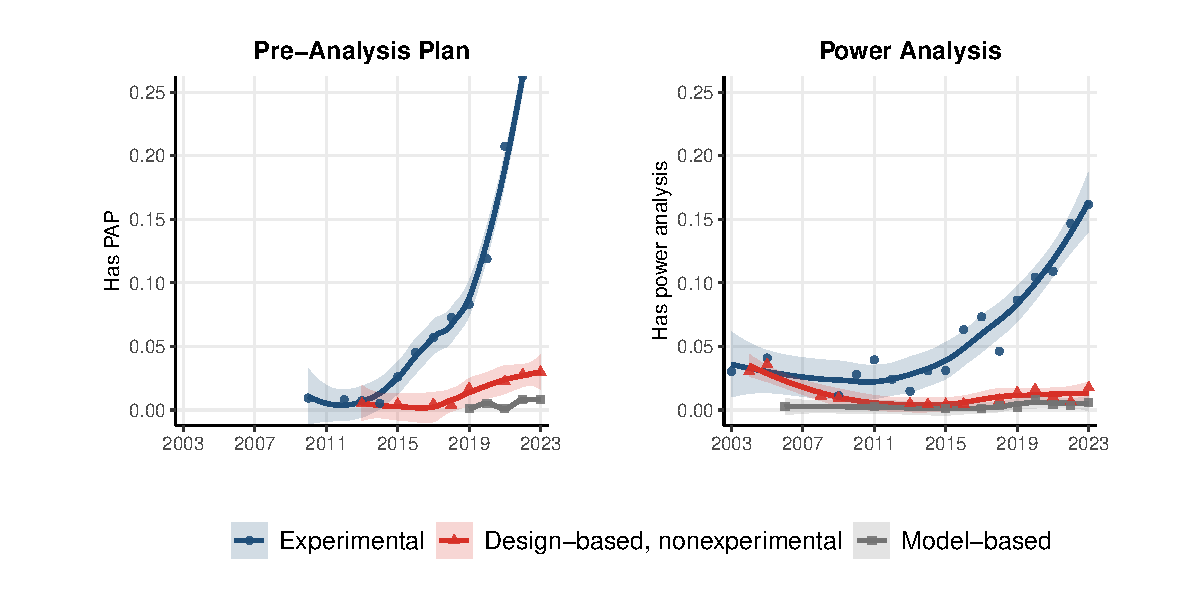
\includegraphics[width=\textwidth]{Figures/qe_notgood_signs.pdf}\vspace{-1em}
    \caption{Best practices for quantitative explanatory papers. Left: proportion reporting pre-analysis plans. Right: proportion reporting power analysis. Experimental, design-based nonexperimental, and model-based studies are in blue, red, and gray, respectively.}
    \label{fig:notgoodsigns}
\end{figure}

Pre-analysis plans show sharp growth but almost exclusively within experimental work, reaching approximately 35\% by 2023. Design-based observational studies exhibit minimal adoption, rising from essentially zero to roughly 3\%. Power analyses follow a similar pattern: growing from 4\% in 2003 to only 15\% in 2023. Power analysis can inform effect size interpretation and null result credibility across research designs, yet it remains rare even in experimental settings where it most commonly appears.

These patterns indicate the credibility revolution has produced an uneven transformation in research practices. Explicit identification assumptions have diffused widely and are now standard practice in design-based research. Other transparency practices, however, remain concentrated in specific method or show limited adoption overall. The credibility revolution has altered how researchers articulate identification strategies, but has not reshaped research standards comprehensively.

\fi

\FloatBarrier

\subsection*{Citation Premium for Design-Based Methods Persists}\label{sec:impact} 

Discipline-wide transformation is reflected not only in shifts in research practices and design choices, but also in changes in what the discipline values and rewards. Citations, despite their limitations, offer one useful proxy: they reflect what gets read, built upon, and treated as influential. Because citation counts affect promotion, hiring, and professional recognition, they provide insight into how the field allocates prestige.

If the credibility revolution reshaped political science, design-based studies might be expected to receive more citations than model-based work. We refer to this difference---the average number of additional citations that design-based papers receive compared to model-based papers published in the same year---as the \emph{citation premium} for design-based studies. A key limitation of this analysis is that we do not account for possible confounders such as topic, subfield, journal placement, or research quality, so these patterns should not be interpreted as causal effects.

\begin{figure}[!ht]
    \centering

    \begin{subfigure}[b]{0.47\textwidth}
        \centering
        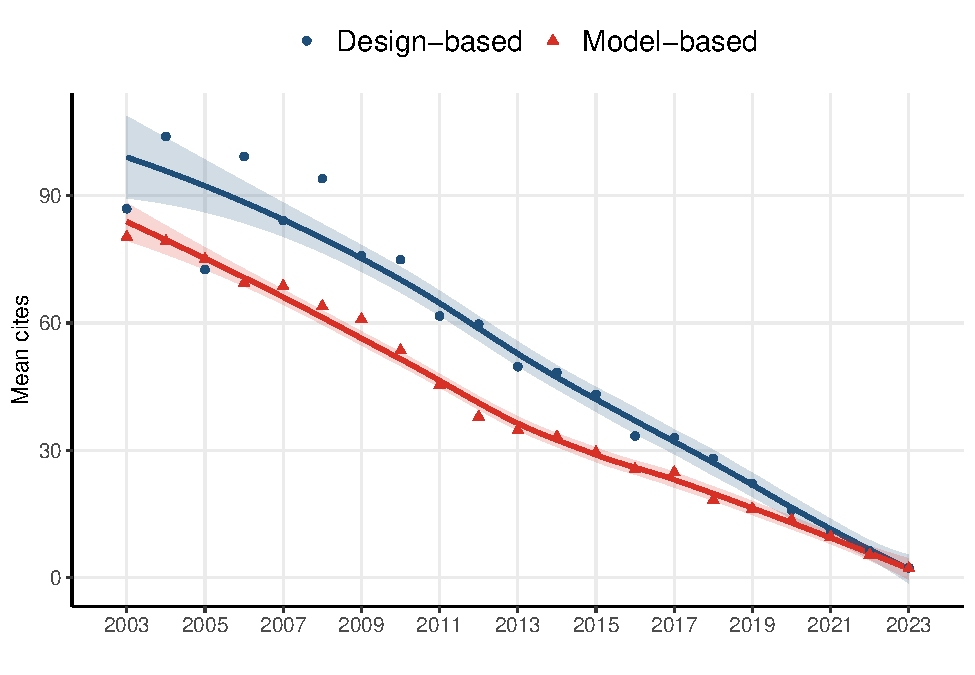
\includegraphics[width=\linewidth]{Figures/qp_cites_by_broad_cat_raw.pdf}
        \caption{Citation count in 2023 by publication year}
        \label{fig:cite.raw}
    \end{subfigure}
    \hfill
    \begin{subfigure}[b]{0.47\textwidth}
        \centering
        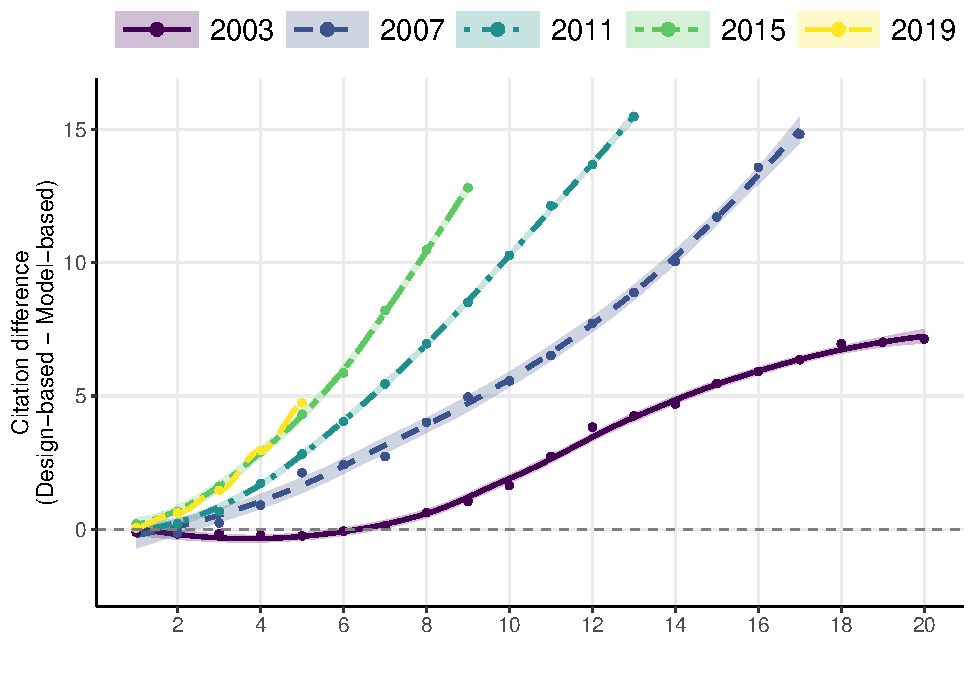
\includegraphics[width=\linewidth]{Figures/qp_cites_trends.pdf}
        \caption{Citation premium by publication year}
        \label{fig:cite.sd}
    \end{subfigure}
\caption{Citation premium for design-based methods. The left panel shows the average citation count for design-based (blue) and model-based (red) studies by publication year in 2023. The right panel shows the citation premium (the difference in average citations between design-based and model-based studies) measured relative to the publication year for papers published in 2003, 2007, 2011, 2015, and 2019.}
    \label{fig:citemeansoverall}
\end{figure}


Comparing citation levels across years is complicated by the fact that citations accumulate over time, so more recent papers have had fewer years to be cited, and design-based methods have become more common in later cohorts. To address these issues, we examine both raw citation counts by publication year and cohort-specific citation trajectories.

Figure~\ref{fig:citemeansoverall}(a) presents the average number of citations received by design-based and model-based papers. The citation premium emerges in the early 2000s, grows through the late 2000s, peaks around 2011, and appears to narrow in more recent years. Two considerations likely contribute to this pattern. First, newer papers have had less time to accumulate citations, which mechanically reduces observable gaps. Second, as design-based methods became more common, including in influential journals, the bar for publishing model-based work may have risen, producing stronger model-based papers in recent years and narrowing the citation differential. In addition, the broader diffusion of design-based approaches means that some studies may adopt these methods uncritically, without fully justifying the required assumptions, limiting their potential to generate a citation advantage.

Figure~\ref{fig:citemeansoverall}(b) shows the citation premium for cohorts of papers published in 2003, 2007, 2011, 2015, and 2019, measured relative to each paper's publication year. The premium is consistently positive, but varies by cohort. The 2003 cohort shows a small advantage of about seven additional citations after twenty years. The 2007 cohort rises more quickly, reaching roughly fifteen extra citations after sixteen years, a pattern matched by the 2011 cohort within eleven years. The 2015 cohort accelerates further, gaining about ten additional citations within eight years, compared to seven for the 2011 cohort at the same point. The 2019 cohort tracks the 2015 pattern closely, suggesting that the premium may have stabilized. 

We complement the descriptive evidence with a regression-based analysis of citation differences between design-based and model-based papers, controlling for subfield, journal, and year fixed effects and for paper and author-level covariates. Results in Table \ref{tab:citation_regression}, confirm the findings shown in Figure \ref{fig:citemeansoverall}: design-based studies receive more citations on average, but the premium is larger for earlier cohorts and attenuates over time. While informative, the regression estimates remain descriptive and should not be interpreted as causal.
 

\FloatBarrier

\section*{Discussion}\label{sec:discussion}

Our analysis paints a mixed picture of the credibility revolution in political science. On the one hand, design-based methods have moved from the margins to rough parity with traditional model-based approaches in quantitative explanatory research. Design-based strategies now account for about 40\% of such papers, and they receive a persistent citation premium relative to model-based work. On the other hand, this transformation is not universal and remains highly stratified. It is disproportionately driven by a single design---survey experiments---and is concentrated in top journals and among authors affiliated with highly ranked institutions. Credibility-enhancing practices beyond research design, such as pre-analysis plans, power analyses, and placebo tests, remain far from universal even among design-based studies. In this sense, the credibility revolution is better described as a substantial but partial reform than as a wholesale reordering of empirical practice.

Several developments are nonetheless incontestable. First, the discipline has become less reliant on parametric modeling as the default route to causal claims. The growth of experiments, regression discontinuity, and other designs has shifted attention from functional form assumptions to explicit statements about treatment assignment and identifying variation. Second, researchers overall are now much more explicit about the assumptions required for causal interpretation: identification assumptions are stated in more than 90\% of design-based papers and in most model-based papers. Third, median sample sizes have increased across methodological families, which, all else equal, should improve statistical power and reduce the risk that published findings are driven by small-sample noise. Together, these changes move the discipline closer to the standards articulated by proponents of the credibility revolution.

Simultaneously, the evidence suggests that the credibility revolution is not deep in at least two respects. First, the adoption of design-based methods is highly concentrated in survey experiments, which account for nearly half of all design-based papers toward the end of the period. Other designs central to the credibility revolution playbook---difference-in-differences, regression discontinuity, natural and quasi-experiments, synthetic control---remain rare and often exhibit non-monotonic usage patterns, suggestive of methodological fashions rather than durable practice. This concentration limits the types of questions that can be credibly addressed and leaves many important settings under exploited. Second, outside of identification assumptions, other credibility-enhancing procedures remain weakly institutionalized. Placebo tests are used in only about one-fifth of design-based observational studies and are very rare elsewhere. Pre-analysis plans and power analyses are mostly confined to experimental work and remain the exception even there. If the goal is to make published evidence more diagnostic of causal claims, these ancillary practices will need to become more routine across methods, not just in a subset of high-profile experiments. %Moreover, clear and precise statements of the exact causal quantity of interest remain uncommon even among design-based studies.

The reach of the credibility revolution is also not wide. Design-based methods were adopted earlier and at higher rates in the discipline's most prestigious journals and among authors at top-ranked institutions. Regression discontinuity designs and field experiments, for example, are disproportionately concentrated in top-10 outlets and in the upper tail of the institutional ranking, whereas adoption rates flatten beyond roughly the top-50 institutions. These patterns are descriptive and likely reflect selection on training, resources, and submission strategies as well as differential ``internalization'' of credibility principles. They nonetheless raise the possibility of a two-tiered discipline in which standards for credible causal inference vary by institutional location. 

The findings we present warrant an important interpretive caveat: because our measures rely on how authors describe their designs and aims, we cannot fully separate changes in research practice from shifts in how scholars present their work. This matters because evolving reporting norms could bias our descriptive trends, leading us to over- or understate the influence of the credibility revolution. For example, if researchers have become more cautious in making causal claims, model-based studies might now include fewer or more qualified causal statements even without substantive changes in practice—potentially causing us to understate change. Conversely, if scholars increasingly describe their work as “descriptive” rather than “explanatory,” the pool of explanatory studies would shrink, inflating the apparent rise of design-based methods in that category. While we cannot directly test these dynamics, any intellectual movement that redefines causality is likely to transform both how causal claims are evaluated and how they are articulated. Importantly, descriptive evidence in Section~\ref{sisec:altexps} of the Supplementary Materials suggests these processes are not the main drivers of our results: the share of explicitly descriptive quantitative studies remains essentially flat over time, and the proportion of model-based studies making causal claims has held steady since at least 2010.

In sum, the credibility revolution is reshaping---but not displacing---other modes of inquiry. Quantitative explanatory research remains a minority, comprising about 41\% of articles in our corpus. Although its share has grown, it has not supplanted the field’s methodological diversity. Our findings point to an emerging equilibrium in which design-based research coexists with, and is enriched by, qualitative, historical, ethnographic, and interpretive approaches, as well as formal and normative theory. As standards for causal inference evolve, the contributions of other traditions—especially their capacity to capture meaning, context, complexity, and contingency—remain essential. Qualitative scholars have long developed tools for causal inference, including process tracing and within-case analysis, that offer alternative logics and forms of evidence. Descriptive work continues to play a vital role in mapping new phenomena, measuring key constructs, and shaping research agendas. From this perspective, the credibility revolution may be most productive when it fosters a division of labor and mutual reinforcement across methods, advancing methodological pluralism rather than elevating any single paradigm.


\pagebreak



% \begin{enumerate}
% \item yes some changes but partial changes
% \item Yes design based is the modal method, but also model based is almost as common
% \item yes survey experiments are most of it but top 10 show maybe we are going to see a change
% \item WE do see evidence of two tier system, where top of the discipline is more design based
% \item beyond research designs other credibility pracitces indeed more popular but again, not nearlly close to universal adoption although trends are promising. 
% \item weird that such a stratification exists btw experimetns and not experiments. 
% \item and there is indeed a citation premium for design, that second derivative is smaller - so maybe it is becoming the new normal
% \item but still levels are not there, intensive and extensive margine are not there for revoltuion. 
% \item yes accounting for what gets readh the disfference is starker but even so reform more than revolution?

% \end{enumerate}

% \newpage 
\vspace{3em}
\onehalfspacing
\bibliography{refs}
\clearpage
%%%%%%%%%%%%%%%%%%%%%%%%%%%%%%%%%%%%%%%%%%%%%%%%%%%


\appendix
\onehalfspacing
\setcounter{page}{1}
\setcounter{table}{0}
\setcounter{figure}{0}
\setcounter{equation}{0}
\setcounter{footnote}{0}
\renewcommand\thetable{A\arabic{table}}
\renewcommand\thefigure{A\arabic{figure}}
\renewcommand{\thepage}{A-\arabic{page}}
\renewcommand{\theequation}{A\arabic{equation}}
\renewcommand{\thefootnote}{A\arabic{footnote}}




%\pagenumbering{roman}
% \thispagestyle{empty}
% \begin{center}
%     \Large
%     {\bf Online Supplementary Materials}
% \end{center}

% \setstretch{1.75}
% \vspace{-24pt}

% {\hypersetup{linkcolor=black} \singlespacing
% 	\startcontents[sections]
% 	\printcontents[sections]{l}{1}{\setcounter{tocdepth}{2}}}
% \vspace{24pt}
% \clearpage


\vspace{0em}
\section{Online Supplementary Materials}
\bigskip
\noindent\vspace{0em}{\bf \underline{Table of Contents}}

\begin{enumerate}\itemsep0ex
    \item[A.1.] Data and Sample
    \item[A.2.] Measures and LLM Pipeline
    \item[A.3.] Additional Results
\end{enumerate}

\bigskip

\subsection{Data and Sample}

\subsubsection*{Data Collection and Access}

Our analysis draws on a comprehensive corpus of political science research assembled for a companion study \citep{grossman2025political}. We briefly describe the dataset and its construction here; full details appear in that paper's appendix.

We began with 188 journals classified as political science by Clarivate's Web of Science platform that have a Scientific Journal Rankings (SJR) score of at least one. An SJR below one substantively means that papers in a journal occupy significantly less visibility  and  impact  than  the  average  paper  in  the  discipline. From this list, we removed journals that were not indexed in Scopus, not peer-reviewed, or not published in English, yielding a final sample of 174 journals. Using the Scopus API, we extracted journal-level metadata---including citation statistics---and article-level information (authors, title, abstract, publication date, and DOI) for all 129,751 articles published in these journals between 2003 and 2023.

Wherever possible---and wherever retrieval was consistent with the Text and Data Mining (TDM) provisions in the terms of service of the publishers (e.g. Taylor \& Francis states: ``If you or your institution subscribes to content from Taylor \& Francis you can carry out [TDM] activities on this content, as well as open access content, without any additional charge, provided this is on a non-commercial basis.'')---we obtained the full text of these articles, accessing them through institutional library subscriptions. We successfully retrieved the complete text for 91,632 articles from 156 journals. Importantly, our use of article text is limited to computational analysis; we do not (and will not) redistribute, republish, or publicly share any of the raw text we retrieved. Table \ref{tab:insample_text} shows the universe of journals included in our full-text sample. 

\setlength\LTleft{0pt}
\setlength\LTright{0pt}

%%%%%%%%%%%%%%%%%%%%%%%%%%%%%%%%%%%%
% In Sample (With Text)
%%%%%%%%%%%%%%%%%%%%%%%%%%%%%%%%%%%%

\begin{longtable}{p{0.32\textwidth}p{0.32\textwidth}p{0.32\textwidth}}
\caption{Journal Sample Composition: In Sample (With Text)}
\label{tab:insample_text} \\
\hline
\textbf{Journal Title} & \textbf{Journal Title} & \textbf{Journal Title} \\
\hline
\endfirsthead
\hline
\textbf{Journal Title} & \textbf{Journal Title} & \textbf{Journal Title} \\
\hline
\endhead
International Organization & Political Communication & American Political Science Review \\
Contemporary Security Policy & Environmental Politics & Political Analysis \\
European Journal of Political Research & British Journal of Political Science & Comparative Political Studies \\
World Politics & Policy and Internet & International Journal of Press/Politics \\
Global Environmental Politics & Political Psychology & Journal of Chinese Political Science \\
Review of International Political Economy & Journal of Public Administration Research and Theory & West European Politics \\
American Journal of Political Science & Journal of European Public Policy & New Political Economy \\
Political Geography & Review of International Organizations & Political Behavior \\
Political Science Research and Methods & Policy Studies Journal & Perspectives on Politics \\
Socio-Economic Review & Journal of Peace Research & Public Administration \\
Canadian Journal of Political Science & Public Opinion Quarterly & International Environmental Agreements \\
Politics and Gender & International Studies Review & International Theory \\
South European Society and Politics & PS: Political Science and Politics & East European Politics \\
Democratization & European Political Science Review & Journal of Democracy \\
Journal of Politics & Journal of Conflict Resolution & Political Studies \\
Social Movement Studies & Regulation and Governance & Journal of European Integration \\
Geopolitics & Governance & African Affairs \\
Government and Opposition & Annals of the American Academy of Political and Social Science & Research and Politics \\
Party Politics & Studies in Comparative International Development & International Studies Quarterly \\
Journal of Information Technology and Politics & Territory, Politics, Governance & Journal of Current Southeast Asian Affairs \\
International Political Sociology & Terrorism and Political Violence & Journal of Public Policy \\
Politics and Society & European Union Politics & Electoral Studies \\
Comparative Politics & Nations and Nationalism & Philosophy and Public Affairs \\
International Political Science Review & Post-Soviet Affairs & Swiss Political Science Review \\
Journal of Common Market Studies & Political Research Quarterly & European Political Science \\
Review of Policy Research & Cooperation and Conflict & European Journal of Political Economy \\
Studies in Conflict and Terrorism & Political Quarterly & Latin American Politics and Society \\
Journal of Strategic Studies & Social Science Quarterly & Local Government Studies \\
Journal of Human Rights & International Journal of Conflict and Violence & New Left Review \\
Politics & Contemporary Political Theory & Publius: The Journal of Federalism \\
Business and Politics & International Journal of Public Opinion Research & Journal of Elections, Public Opinion and Parties \\
British Journal of Politics and International Relations & Citizenship Studies & Journal of Political Philosophy \\
Mediterranean Politics & Journal of International Relations and Development & Quarterly Journal of Political Science \\
Comparative European Politics & European Security & International Journal of Transitional Justice \\
International Feminist Journal of Politics & Problems of Post-Communism & Public Choice \\
American Politics Research & Legislative Studies Quarterly & Europe-Asia Studies \\
German Politics & International Politics & Armed Forces and Society \\
Political Theory & Review of African Political Economy & Journal of Contemporary European Studies \\
Scandinavian Political Studies & Ethics and International Affairs & Current History \\
International Affairs & Political Science & Intelligence and National Security \\
Nationalities Papers & Acta Politica & Parliamentary Affairs \\
Survival & Australian Journal of Political Science & Revista Brasileira de Política Internacional \\
Journal of Women, Politics and Policy & British Politics & Scottish Journal of Political Economy \\
Polity & Japanese Journal of Political Science & Journal of Theoretical Politics \\
Economics and Politics & Human Rights Quarterly & Contemporary Southeast Asia \\
Politics, Philosophy and Economics & Communist and Post-Communist Studies & Australian Journal of Politics and History \\
Presidential Studies Quarterly & Critical Review & Political Science Quarterly \\
Studies in American Political Development & Forum & East European Politics and Societies \\
Latin American Perspectives & Irish Political Studies & Ethics and Global Politics \\
Historical Materialism & European History Quarterly & Politická ekonomie \\
Journal of Policy History & Telos & \\

\hline
\end{longtable}
\clearpage

\subsubsection*{SCImago Journal Rank}

SJR (SCImago Journal Rank) is a metric used in Scopus to assess the impact and prestige of
academic journals. A key feature of SJR is that it is a Prestige-Weighted Metric: it measures
the scientific influence of journals by considering both the number of citations they receive
and the prestige of the journals where those citations come from. Unlike raw citation counts,
SJR assigns higher value to citations from more influential journals. Specifically, SJR is the
number of citations in a specific year (e.g., 2023) to articles published in the previous three
years (e.g., 2020–2022), considering the prestige of the citing journals.



\subsubsection*{Sample Construction}

Table \ref{tab:sankey} reports the sample construction, reported in Figure \ref{fig:sankey} in the main text. Each panel corresponds to a classification stage. Of the 91,632 papers in our corpus, 37,163 (40.6\%) are classified as quantitative empirical. Among these, 30,290 (81.5\%) are coded as having an explanatory goal. Last, Panel C breaks down the explanatory papers by identification strategy.

\begin{table}[htbp]
\centering
\begin{small}
\begin{tabular}{@{}lrc@{}}
\toprule
 & N & \% \\
\midrule
\multicolumn{3}{@{}l}{\textbf{Panel A: All studies (N = 91,632)}} \\
\quad Quantitative empirical & 37,163 & 40.6 \\
\quad Not quantitative & 54,469 & 59.4 \\
\addlinespace
\multicolumn{3}{@{}l}{\textbf{Panel B: By goal (N = 37,163)}} \\
\quad Explain & 30,290 & 81.5 \\
\quad Describe & 6,633 & 17.8 \\
\quad Predict & 240 & 0.6 \\
\addlinespace
\multicolumn{3}{@{}l}{\textbf{Panel C: By method (N = 30,290)}} \\
\quad Design-based methods & 8,695 & 28.7 \\
\quad Model-based methods & 15,863 & 52.4 \\
\quad Other & 5,732 & 18.9 \\
\bottomrule
\end{tabular}
\end{small}
\caption{Sample construction}
\label{tab:sankey}
\end{table}


\clearpage

\subsection{Measures and LLM Pipeline}

\subsubsection*{Full GPT Prompt Used for Article Classification}\label{sisec:prompt}

The full classification prompt and the associated JSON Schema are provided a below. All logic, definitions, variable names, conditional requirements, and enumeration options are preserved exactly as used during classification. A full list of variables coded by the prompt is shown in table \ref{tab:prompt_variables}.

{\scriptsize
\begin{Verbatim}[breaklines=true]
TASK OVERVIEW

You are an expert-level political science paper analysis engine, a domain‑expert engine that reads political‑science manuscripts and classifies them into a series of variables. You must: interpret complex academic content, focusing on research methods, causal claims, data usage, measurements, identification strategies, use domain knowledge to classify subfields, and more.

Your tasks:

-   Read and understand the entire provided paper -- title, abstract, main text, tables/figures, footnotes, etc.

-   Identify the strongest evidence and framing -- focus on the headline findings that the authors highlight.

-   Extract and return the metadata described below, obeying the interpretation rules for each, and responding according to the JSON schema provided.

Note: If a property's type includes "null" (e.g., ["boolean","null"] or ["array","null"]), use null if and only if information in the paper is missing or it the specific variable is not applicable to the study design (e.g. parallel trends assumption isn't relevant to a survey experiment)

Specific instructions and definitions for each property are outlined below:

0. error_in_raw_text: first, before anything else, confirm that the Paper Full TEXT makes sense in regards to the Paper Title. Specifically, pay attention to the fact that the raw text might be specified or corrupt. Select from the following options.

    - No Error — this is if the raw text seems okay.

    - Missing/Corrupt — this is if the raw text is totally missing or unreadable. Note, it is okay if the text is just messy; this variable is reserved for totally broken texts and NaNs.

    - Title/Text Mismatch — this is if it is *obvious* that the raw text does not match the title. For example, if the paper title is talking about Elections in Africa but the paper is about Gender in US Congress, obviously something has gone wrong. It should be very clear if this type of mismatch has occurred.

1.  subfield: Select of the enumerated canonical Political Science subfields that the paper best fits into. Most papers should fall into one of these, but choose 'Other' if truly uncertain. Canonical definitions:

    - American Politics: Empirical or historical study of political behavior, institutions, or processes inside the United States (e.g. Congress, presidency, courts, elections, parties, public opinion, state policy, race/ethnicity and politics, federalism, etc.).

    - Comparative Politics: Comparative Politics: Systematic comparison across sovereign states, sub-national units (states, provinces, districts, etc.), non-state actors that play an important political role (churches, NGOs, traditional authorities like chiefs, etc), or general inference drawn from non-U.S. politics (e.g. regime type, democratization, comparative institutions, political economy, civil conflict within states, elections outside the U.S., etc.).

    - International Relations: Analysis of cross-border political interactions such as interstate conflict and cooperation, trade, international organizations (such as WHO, WTO, IMF), global governance, global public goods, diplomacy, international political economy, transnational actors, security studies (including, but not limited to nuclear proliferation, military alliances, and technology and weaponry). Also include public opinion surveys and survey experiments that seek to capture opinions of the public or elites toward foreign policy and how they influence foreign policy making.

    - Methodology and Formal Theory – Research that develops or critiques analytical methods, measurement, statistics, or formal (game-theoretic) models for broad disciplinary use.

    - Political Theory and Philosophy – Normative reasoning, conceptual analysis, or interpretation of classic and contemporary texts.

    - Public Policy/Administration – Study of policy design, implementation, and evaluation, and bureaucratic behavior within governmental systems. Public administration generally focuses on practical aspects of managing and implementing public policies, programs, and services. For example, it explores the pros and cons of different ways to organize the bureaucracy and its implication for effective delivery of public services, and ensuring that laws and regulations are effectively executed. 

    - Other – Assigned when paper doesn't fit into any subfield or the work lies entirely outside political science.

2.  is_empirical_quant_paper: true if the paper contains any original data analysis using quantitative methods, descriptive, predictive, causal, or other. False if the paper uses empirical qualitative methods (e.g. case studies, process tracing, etc), normative, theory, etc. If this is false, most of the subsequent variables are no longer applicable and should be null.

3.  general_goal_of_analysis: is_empirical_quant_paper == FALSE, this is "null". Otherwise, read the paper and interpret its high level approach. Specifically, code what the 'goal' of the analysis in the paper is in terms of the three distinct categories below. Note, this is not about the design of the paper per say, but more about the question it is trying to answer / its purported motivation.

    - Describe: A paper which seeks to describe a phenomenon that occurs in the world, understand its baseline levels, differences across groups etc. It doesn't seek to explain it, but merely describes something, its nature, its degree, etc. A descriptive analysis.

    - Predict: A paper which seeks to predict an outcome based on a set of variables or determine which variables are most predictive of a perceived relationship, albeit not assuming those variables are the cause/consequence of the relationship. A predictive analysis.

    - Explain: A paper which seeks to actually explain a phenomenon/relationship and identify the causes or consequences of the said phenomenon/relationship. The paper is motivated by a desire to identify a causal effect in the universe (regardless of whether it actually succeeds in this). Its goal is to make an inference. A causal analysis.

4a. single_country_study: is the main analysis of this paper focused on a single country?  Select one of: single_country, multiple_countries, or NA if not relevant (e.g. a paper talking only about methods).

4b. single_region: if single_country_study is “multiple_countries”, then select one of: single_region, multiple_region, otherwise leave as null if not “multiple_countries”. single_region should be selected if all countries that are the focus of the main analysis of the paper are from the same global region. Regions are defined as follows: East Asia & Pacific, Europe & Central Asia, Latin America & Cuba, Middle East & North Africa, North America, South Asia, Sub-Saharan Africa.

5. countries_of_focus: enumerate the countries examined in the primary analysis of the paper, their names separated by semicolons. If there is a single country, just return the name of that country. If there are greater than 20 distinct countries, then return “20+ Countries” instead of a complete list.

6. paper_uses_survey_data: does the paper use survey data for its primary analysis? Return one of: no_survey_data, runs_original_survey, uses_public_available_survey (e.g. Afrobarometer, ANES, data from a previously published paper, etc.)

7. uses_original_dataset: if the authors use an original dataset for their paper’s primary analysis, write the type used here. Importantly, the focus here is only the primary independent or dependent variables in the main analysis. Null if the paper doesn't use any data at all. Options follow:

    - original_survey: if the researchers design and field an original survey

    - field_experiment: if the researchers run a field experiment with a treatment produced by the researchers

    - field_study: non-experimental, original, primary data gathering in the field, thus creating a new dataset that didn't exist before

    - structure_systematize: if the researchers take unstructured information and structure/systematize it into usable data (e.g. text-as-data). Note this does not include the manipulation of variables in existing datasets, but rather it must begin with unstructured, non-data information that the authors themselves parse/structure

    - procure_original_data: if the researchers procure, for example, via a FOIA request, data/information heretofore private or unused by other researchers

    - other_original_data: if the researchers use truly original data that doesn't fall into the above categories (e.g. biometric data collected via wearable devices, sensor data from custom-built hardware,  behavioral lab setups not qualifying as a field experiment, etc)

    - not_original: if the researchers use existing datasets, publicly available surveys, combining datasets to create new measures, etc. it does not count as original

8. seeks_determinants: true if a) the paper is an "Explain" paper (null if "Predict" or "Describe") and b) the purported goal of the paper is to investigate which observable factors explain variation in a specific outcome variable observed in the world — in other words, the determinants of a given variable. In other words, if the paper’s primary goal is to quantify how factors jointly or individually drive an outcome, distinct from estimating the effect of a researcher‐defined treatment. Note: do not include papers that specifically explore determinants to treatment assignment in an effort to make a more credible causal argument (often combined with a selection-on-observables assumption); these are ancillary balance or selection checks rather than a substantive determinants inquiry.

9.  main_causal_research_design: select the research design the papers uses to generate the primary causal claim in the paper. Treat "Other" as catch‑all when none of these specific designs apply. If there are multiple categories from the given list, select "Multiple Designs" and list them in "other_research_design". If general_goal_of_analysis is "Describe" or "Predict", then leave this field "null". Use the following canonical research design definitions

    - Field Experiment: Researcher‐implemented random assignment of treatment in participants’ real-world environment (schools, firms, markets, governments, etc.). Setting is natural. Exclude survey-based or lab settings.

    - Survey Experiment: Random assignment is embedded inside a survey instrument (question wording, vignettes, information treatments, conjoint tasks). Sampling frame is a survey panel or similar; the experiment exists only within the survey session. Exclude field experiments that merely measure outcomes with a survey.

    - Lab Experiment: Random assignment conducted in an artificial, researcher-controlled environment (physical lab or online platform designed to mimic a lab). Tight control over information, incentives, timing; participants act under awareness of being studied.

    - Difference-in-Differences (Diff-in-Diff): Quasi-experimental panel or repeated-cross-section design comparing changes over time between treated and untreated groups. Identification comes from the interaction of post period and treated groups, under the parallel-trends assumption. Implementations may include two-way fixed effects, event studies, staggered adoption corrections, or synthetic DID weights, but a common-trend contrast is the core.

    - Instrumental Variable (IV): Uses an exogenous instrument ZZZ that shifts treatment DDD while affecting the outcome YYY only through DDD (relevance + exclusion). Primary estimator is two-stage least squares, control-function, or equivalent; the estimand is a Local Average Treatment Effect for compliers. Exclude designs where the “instrument” is actually a cutoff (RDD) or time variation (Diff-in-Diff).

    - Regression Discontinuity Design (RDD): Exploits a discrete jump in treatment assignment/assignment probability at a known cutoff of a running variable. Identification comes from continuity of potential outcomes at the threshold; effect is estimated via local linear/polynomial or bias-corrected methods. Exclude kink designs (slope change) and IV interpretations of cutoffs.

    - Regression Kink Design (RKD): Exploits a deterministic change in the slope (kink) of the treatment rule at a threshold. Identification uses the change in the derivative of the outcome with respect to the running variable. Requires smoothness of potential outcomes’ first derivative. Distinct from RDD because treatment probability is continuous at the threshold.

    - Synthetic Control: Constructs a weighted combination of control units to replicate the treated unit’s pre-intervention path; the post-intervention gap yields the causal effect. Key features: donor-pool weighting constrained to pre-period fit, usually a single treated unit or small set. Exclude simple matching or DiD unless weights are chosen to replicate pre-trends without parametric regression.

    - Matching/Balancing/Weighting: explicitly invoke the unconfoundedness assumption (also known as ignorability or selection-on-observables) with explicit construction of comparable treatment and control groups through matching, weighting, or balancing techniques. Such methods include: covariate matching, exact matching, generic matching, coarsened exact match, nearest-neighbor matching, entropy balancing, kernel balancing, propensity score matching, propensity score balancing, propensity score matching, inverse propensity score weighting (IPW), augmented inverse propensity score weighting (IPW), and covariate-balancing propensity score. Identification hinges on both unconfoundedness and the overlap assumption. Overlap means the similarity of the treatment and control groups in terms of their covariates. Assessing overlap is often based on propensity scores or a balance table. Exclude designs that also exploit an IV, cutoff, staggered timing, or panel differential trends—those fall under IV, RDD, DiD, etc. This is distinct from the Kitchen Sink Linear Model given the critical thought required to implement the selection-on-observables w/ matching/weighting/balancing techniques & assessing overlap vs a “throw-everything-in” approach.

    - Kitchen Sink Linear Model: OLS/Logit/etc. with a treatment indicator and an extensive vector of covariates chosen ad-hoc or “throw-everything-in”, but without an explicit, theory-based identification design (no instrument, cutoff, policy shock, or parallel-trend justification). Causal claim relies solely on conditional-independence/selection-on-observables.

    - Multiple Designs: Paper deploys two or more distinct causal designs (from this list) as complementary, co-equal strategies for the same causal question (e.g., RDD + IV robustness, or RDD plus Diff-in-Diff).

10.  other_research_design: If general_goal_of_analysis == "Describe" or "Predict" or main_causal_research_design = "Other" / "Multiple Designs", enter a concise label for the design used here; else null.

11. instrumental_variable_instrument: If main_causal_research_design is "Instrumental Variable", give a concise name for the variable used as an instrument in the analysis. If not an "Instrumental Variable" analysis, then null.

12. placebo_test: TRUE if the article engages in a formal, quantitative placebo test using data. A placebo test is a statistical test in which researchers either (a) use an outcome known not to be affected by the treatment and test the treatment’s effect on this placebo outcome, or (b) use a treatment known to have zero effect on the outcome and test its effect on the outcome. Ideally, the placebo test should return a null effect. The goal of placebo tests is to assess whether the key assumption is plausible. FALSE otherwise. 

13.  independent_variables and dependent_variables: List the key variables used in main research design. Each must have a *variable_name* and a *variable_description*. For variable names, be as concise and general. For example, if the paper is using incumbent vote-share from municipal elections in Brazil in 2016, just call that 'Vote Share' and leave the details for the variable_description. If this IV/DV framework is not relevant to the paper in question, leave as "null" instead of as an array.

14.  main_variable_relationship: Create one element per primary IV→DV pair discussed in the headline findings. Use names consistent with the variables above. Identify the direction of the relationship (relationship_type: "Positive", "Negative", "Non-Monotonic", "null", or "Unknown") and whether it was statistically_significant / substantively_significant (to determine significance significance, rely on authors' language rather than on the numbers, since the numbers/tables in the paper's raw text is unlikely to be parsed correctly). If this framework is not relevant to the paper in question, leave as "null" instead of as an array.

15.  makes_explicit_causal_claim: a boolean value coding whether the paper makes an *explicit* causal claim regarding the primary independent variable. Note, this is specific to the primary analysis/main result of the paper; do not consider ancillary analyses or statements that reference known causal relationships outside the scope of the paper (e.g. citing a difference paper or theorizing in the introduction). "Explicit" means that the paper states the causal relationship explicitly (e.g. "A causes B", "the [key independent variable] caused an x% increase to the [DV]", "the impact of the [key independent variable] on the [DV] is x", "the effect of the [key independent variable] on the [DV] is x", “This article shows the effects of...",  “Table X shows the effect of...”, “___ seems to have been a stronger determinant of ___”, etc.) Other expressions that indicate an explicit causal claim when used to describe the relationship between the focal variables include: "increase", "decrease", "reduce", "diminishes", "lead to", "result in", "impact", "influence", "affect", "elevate", and similar terms.

16.  makes_implicit_causal_claim: a boolean value coding whether the paper makes an *implicit* causal claim regarding the primary independent variable. This is often the case in papers where the authors try to tone down causal language by using non-causal language for the key explanatory variable despite the fact that the paper is organized/oriented as if it were exploring a causal relationship between two variables. Even though these papers avoid causal language, the paper relies on implicit causality to support the theory or mechanism. FALSE if makes_explicit_causal_claim is TRUE.

17. strong_non_causal_causal_qualification: a boolean value coding whether the paper explicitly states that the relationship between the primary independent variables and the outcomes of interest are not causal. Note: strong_non_causal_causal_qualification and makes_implicit_causal_claim causal claim can both be TRUE if the paper implicitly still frames itself causally (i.e. the qualification is not totally sincere). For example:
    - “The analysis is correlational and should not be interpreted as causal”
    
    - “These associations do not imply causation.”
    
    - “Findings are not evidence of causal impact.”
    
    - “Results cannot establish causal direction.”
    
    - “Observed linkages are descriptive rather than causal.”
    
    - “The estimates indicate association; claims of causality would be premature.”
    
    - “Data limitations preclude definitive causal conclusions.”
    
    - “This research identifies patterns, not causal effects.”
    
    - etc.

18. sample_size: if relevant to the paper, try to identify the sample size used in the main analysis. If there are multiple, do not try to combine/aggregate the sample sizes, but instead, use your judgement to identify the primary sample N. Often this is the sample size reported in the table or figure showing the paper's main result. Note: sample size is defined at the unit of observation (e.g. a study of 50 countries across 10 years would probably be a 500 country-year sample size, not 50). Do NOT make up any numbers; it is better to return 'null' than a false value.

19. sample_size_quote: to prove that you are not hallucinating the sample_size value above, please include the exact one-sentence quote/line from the paper which you used to retrieve the sample size. If you are unable to identify this line, then reconsider whether your sample_size coding above is legitimate.

20. claims_any_statistically_significant_results: true if the main result is claimed by the author to be statistically significant. false if not.

Design‑clarity and rigor flags:

21. references_power_analysis: true if the authors reference/report a power analysis. Note: this is true even if the power calculations are only reported in the appendix/pre-analysis plan, as long as the author indicates that they considered statistical power. Else false.

22. clearly_defined_explanatory_variable: when the paper is seeking to Explain, this is true if the paper clearly states which variable(s) it is focusing on to explain the focal relationship and if it discusses the theoretical underpinning behind using said variable(s).

23. clear_causal_quantity_of_interest: write out the causal quantity of interest if the paper states it directly. If the paper does not clearly state a causal quantity of interest listed below, return "FALSE". If the paper is not causal and thus a causal quantity of interest is irrelevant, return "null". You can ONLY select from the list of causal quantities below. Do not make up/write any other causal quantities.
    
    - ATE – Average Treatment Effect
    - ATT – Average Treatment Effect on the Treated
    - ATC – Average Treatment Effect on the Controls
    - SATE – Sample Average Treatment Effect
    - SATT – Sample Average Treatment Effect on the Treated
    - SATC – Sample Average Treatment Effect on the Controls
    - PATE – Population Average Treatment Effect
    - CATE – Conditional Average Treatment Effect
    - ITE – Individual Treatment Effect
    - LATE – Local Average Treatment Effect
    - CACE – Compiler Average Causal Effect
    - LATT – Local Average Treatment Effect on the Treated
    - LATC – Local Average Treatment Effect on the Controls
    - LIV Effect – Local Instrumental-Variable Treatment Effect
    - PRTE – Policy-Relevant Treatment Effect
    - MTE – Marginal Treatment Effect
    - QTE – Quantile Treatment Effect
    - CQTE – Conditional Quantile Treatment Effect
    - LQTE – Local Quantile Treatment Effect
    - TOT – Treatment-on-the-Treated Effect (IV context)
    - ITT – Intention-to-Treat Effect
    - ITTD – Intention-to-Treat Effect on the Difference in outcomes
    - Per-Protocol Effect
    - As-Treated Effect
    - NDE – Natural Direct Effect
    - NIE – Natural Indirect Effect
    - ACME – Average Causal Mediation Effect
    - CDE – Controlled Direct Effect
    - PSE – Path-Specific Effect
    - SACE – Survivor Average Causal Effect
    - PSACE – Principal-Stratum Average Causal Effect
    - APE – Average Partial Effect
    - ASF – Average Structural Function
    - DRF – Dose-Response Function (marginal causal curve)
    - MSM Effect – Marginal Structural Mean Effect
    - RD – Risk Difference (causal)
    - RR – Risk Ratio (causal)
    - OR – Odds Ratio (causal)
    - HR – Hazard Ratio (causal)
    - DiD-ATE – Difference-in-Differences Average Treatment Effect on the Treated
    - Dynamic Treatment Effect (DTE) – Time-varying causal effect path
    - Event-Study ATT – Dynamic DiD causal path
    - SCATE – Synthetic-Control Average Treatment Effect
    - RDD Cut-off Effect – Regression Discontinuity Treatment Effect at threshold
    - RKD Slope Effect – Regression Kink Treatment Effect
    - Spillover Effects – Direct Spillover Effect (DSE), Indirect Spillover Effect (ISE), Total Spillover Effect (TSE)
    - NATE – Network Average Treatment Effect
    - CLATE – Cluster Average Treatment Effect

24. specifies_estimate_equations: true if the paper states/references the actual equation that they are using to run their analysis, making it clear to the reader exactly what they are estimating. False otherwise.

22. discusses_threats_to_causality: true if clear and substantive discussion of possible threats to identifying a causal relationship between the primary IV and DV. Specifically in terms of why it might be, in general, difficult to identify a causal relationship between the primary variables of interest. For example, discussions of exogeneity/endogeneity, self-selection, selection effects, omitted variable bias, reverse causality, survivorship, spillover effects, etc.

23a. statement_of_identification_assumptions_quote: extract the exact quote/sentence-snippets from the text where the identification assumptions defined in 23b below are mentioned. Write 2-3 sentences/sentence snippets maximum. Focus on just the snippet(s) where the specific assumptions are mentioned.

23b. statement_of_identification_assumptions: code true or false whether the paper clearly stated and explicitly discussed the appropriate identification assumptions for the paper’s design. The specific assumptions for each relevant design are enumerated below.

- Field Experiment: Random assignment, Unconfoundedness, SUTVA, Low attrition, No/limited spillover

- Survey Experiment: Random assignment of survey stimulus, No systematic non-response, SUTVA

- Lab Experiment: Random assignment; SUTVA, No uncontrolled environmental or demand effects influencing assignment or outcomes

- Difference-in-Differences (Diff-in-Diff or DID): Parallel trends, Treated and control groups would have identical time-path changes in outcomes, No anticipation effect

- Instrumental Variable (IV): Relevance (or strong instrument), Exclusion Restriction, Independence/unconfoundedness, Monotonicity for LATE

- Regression Discontinuity Design (RDD): Continuity of potential outcomes at cutoff, No precise manipulation of running variable around cutoff, Balanced on covariates around the cutoff

- Regression Kink Design (RKD): Continuity of the slope of potential outcomes in running variable, Kink in treatment rule occurs only at known threshold, No manipulation near kink

- Synthetic Control: Weighted combination of controls replicates treated unit’s pre-treatment outcomes, low-rank structure, No uncontrolled time-varying confounders, No post-treatment shocks unique to controls, No anticipation effect, No major structural changes 

- Matching/Balancing/Weighting: Unconfoundedness given observed covariates, Common support of covariate distributions (also known as overlap or positivity)

- Kitchen Sink Linear Model: Exogeneity of the error term, No perfect multicollinearity, Correct functional form for identification

24. effort_to_explore_mechanisms: Check if the paper devotes a discrete section—or equivalent substance—to exploring the channel/mechanism through which the main IV affects the DV. Note, this does NOT include theoretical discussions at the beginning of the paper, as it must be a discussion which occurs after the main analysis has already yielded results. Options for coding follow:
 
   - "No Mention of Mechanisms/Channels": No mention of mechanisms/channels.

    - "Mechanisms/Channels Mentioned But Not Explored": Mention of mechanisms/channels as passing remarks, conjecture, or future-work notes without data or structured argument.

    - "Mechanisms/Channels Mentioned With Substantial Exploration": (a) a fully articulated discussion of mechanisms/channels to explain the result (more substantial than a passing mention) or (b) a full empirical or formal analysis, such as mediation analysis or exploration of subgroup heterogeneity designed to discriminate mechanisms. 

25. mentions_pre_registered_design_and_analysis_plan: true if the paper mentions that it has been pre-registered or that a pre-analysis plan exists.

<!--begin excerpt-->
Paper Title: 
{TITLE}
==============================
Paper Full TEXT: 
{FULL_TEXT}
<!--end excerpt-->

You are given the full text of a political science paper above. Read it carefully. Then extract the requisite fields following the system guidelines, returning them in valid JSON that satisfies every element of the provided schema. 

\end{Verbatim}
}
\vspace{1em}

{\scriptsize
\begin{Verbatim}[breaklines=true]
json_schema = {
    "json_schema": {
        "type": "json_schema",
        "json_schema": {
            "name": "paper_data_extraction",
            "strict": True,
            "schema": {
                "type": "object",            
                "properties": {
                    "error_in_raw_text": {
                        "type": "string",
                        "enum": [
                            "No Error",
                            "Missing/Corrupt",
                            "Title/Text Mismatch",
                        ]
                    },
                    "subfield": { 
                        "type": "string",
                        "enum": [
                            "American Politics",
                            "Comparative Politics",
                            "International Relations",
                            "Methodology and Formal Theory",
                            "Political Theory and Philosophy",
                            "Public Policy/Administration",
                            "Other"
                        ]
                    },
                    "is_empirical_quant_paper": {"type": "boolean"},
                    "general_goal_of_analysis": {
                        "type": "string", 
                        "enum": [
                            "Describe",
                            "Predict",
                            "Explain",
                            "null"
                        ]
                    },
                    "single_country_study": {
                        "type": "string", 
                        "enum": [
                            "single_country",
                            "multiple_countries",
                            "null"
                        ]
                    },
                    "single_region": {
                        "type": "string", 
                        "enum": [
                            "single_region",
                            "multiple_region",
                            "null"
                        ]
                    },
                    "countries_of_focus": {"type": "string"},
                    "paper_uses_survey_data": {
                        "type": "string", 
                        "enum": [
                            "no_survey_data",
                            "runs_original_survey",
                            "uses_public_available_survey"
                        ]
                    },
                    "uses_original_dataset": {
                        "type": "string", 
                        "enum": [
                            "original_survey",
                            "field_experiment",
                            "field_study",
                            "structure_systematize",
                            "procure_original_data",
                            "other_original_data",
                            "not_original",
                            "null"
                        ]
                    },
                    "seeks_determinants": {"type": ["boolean", "null"]},
                    "main_causal_research_design": {
                        "type": "string", 
                        "enum": [
                            "Field Experiment",
                            "Survey Experiment", 
                            "Lab Experiment",
                            "Diff-in-Diff", 
                            "Instrumental Variable", 
                            "Regression Discontinuity Design",
                            "Regression Kink Design",
                            "Synthetic Control",
                            "Matching/Weighting/Balancing",
                            "Kitchen Sink Linear Model",
                            "Multiple Designs",
                            "Other",
                            "null"
                        ]
                    },
                    "other_research_design": {"type": ["string", "null"]},
                    "instrumental_variable_instrument": {"type": ["string", "null"]},
                    "placebo_test": {"type": ["boolean", "null"]},
                    "independent_variables": {
                        "type": ["array", "null"],
                        "items": {
                            "type": "object",
                            "properties": {
                                "variable_name": {"type": "string"},
                                "variable_description": {"type": "string"}
                            },
                            "required": ["variable_name", "variable_description"],
                            "additionalProperties": False
                        }
                    },
                    "dependent_variables": {
                        "type": ["array", "null"],
                        "items": {
                            "type": "object",
                            "properties": {
                                "variable_name": {"type": "string"},
                                "variable_description": {"type": "string"}
                            },
                            "required": ["variable_name", "variable_description"],
                            "additionalProperties": False
                        }
                    },
                    "main_variable_relationship": {
                        "type": ["array", "null"],
                        "items": {
                            "type": "object",
                            "properties": {
                                "iv_var_name": {"type": "string"},
                                "dv_var_name": {"type": "string"},
                                "relationship_type": {"type": "string", "enum": ["Positive", "Negative", "Non-Monotonic", "Null", "Unknown"]},
                                "statistically_significant": {"type": "boolean"},
                                "substantively_significant": {"type": "boolean"},
                            },
                            "required": ["iv_var_name", "dv_var_name", "relationship_type", "statistically_significant", "substantively_significant"],
                            "additionalProperties": False
                        },
                    },
                    "makes_explicit_causal_claim": {"type": ["boolean", "null"]},
                    "makes_implicit_causal_claim": {"type": ["boolean", "null"]},
                    "strong_non_causal_causal_qualification": {"type": ["boolean", "null"]},
                    "sample_size": {"type": ["integer", "null"]},
                    "sample_size_quote": {"type": ["string", "null"]},
                    "claims_any_statistically_significant_results": {"type": ["boolean", "null"]},
                    "references_power_analysis": {"type": ["boolean", "null"]},
                    "clearly_defined_explanatory_variable": {"type": ["boolean", "null"]},
                    "clear_causal_quantity_of_interest":  {"type": ["string", "null"]},
                    "specifies_estimate_equations": {"type": ["boolean", "null"]},
                    "discusses_threats_to_causality": {"type": ["boolean", "null"]},
                    "statement_of_identification_assumptions_quote": {"type": ["string", "null"]},
                    "statement_of_identification_assumptions":{"type": ["boolean", "null"]},
                    "effort_to_explore_mechanisms": {
                        "type": "string", 
                        "enum": [
                            "No Mention of Mechanisms/Channels",
                            "Mechanisms/Channels Mentioned But Not Explored", 
                            "Mechanisms/Channels Mentioned With Substantial Exploration",
                            "null"
                        ]
                        },
                    "mentions_pre_registered_design_and_analysis_plan": {"type": ["boolean", "null"]},
                },
                "required": [
                    "error_in_raw_text",
                    "subfield",
                    "is_empirical_quant_paper",
                    "general_goal_of_analysis",
                    "single_country_study",
                    "single_region",
                    "countries_of_focus",
                    "paper_uses_survey_data",
                    "uses_original_dataset",
                    "seeks_determinants",
                    "main_causal_research_design",
                    "other_research_design",
                    "instrumental_variable_instrument",
                    "placebo_test",
                    "independent_variables",
                    "dependent_variables",
                    "main_variable_relationship",
                    "makes_explicit_causal_claim",
                    "makes_implicit_causal_claim",
                    "strong_non_causal_causal_qualification",
                    "sample_size",
                    "sample_size_quote",
                    "claims_any_statistically_significant_results",
                    "references_power_analysis",
                    "clearly_defined_explanatory_variable",
                    "clear_causal_quantity_of_interest",
                    "specifies_estimate_equations",
                    "discusses_threats_to_causality",
                    "statement_of_identification_assumptions_quote",
                    "statement_of_identification_assumptions",
                    "effort_to_explore_mechanisms",
                    "mentions_pre_registered_design_and_analysis_plan"
                ],
                "additionalProperties": False
            }
        },
    }
}

\end{Verbatim}
}

\vspace{1em}

\begin{table}[!ht]
\centering
\caption{List of Variables Coded By Prompt \ref{sisec:prompt}}
\label{tab:prompt_variables}
\begin{tabular}{l}
\hline\hline\scriptsize
error\_in\_raw\_text \\
subfield \\
is\_empirical\_quant\_paper \\
general\_goal\_of\_analysis \\
single\_country\_study \\
single\_region \\
countries\_of\_focus \\
paper\_uses\_survey\_data \\
uses\_original\_dataset \\
seeks\_determinants \\
main\_causal\_research\_design \\
other\_research\_design \\
instrumental\_variable\_instrument \\
placebo\_test \\
independent\_variables \\
dependent\_variables \\
main\_variable\_relationship \\
makes\_explicit\_causal\_claim \\
makes\_implicit\_causal\_claim \\
strong\_non\_causal\_causal\_qualification \\
sample\_size \\
sample\_size\_quote \\
claims\_any\_statistically\_significant\_results \\
references\_power\_analysis \\
clearly\_defined\_explanatory\_variable \\
clear\_causal\_quantity\_of\_interest \\
specifies\_estimate\_equations \\
discusses\_threats\_to\_causality \\
statement\_of\_identification\_assumptions\_quote \\
statement\_of\_identification\_assumptions \\
effort\_to\_explore\_mechanisms \\
mentions\_pre\_registered\_design\_and\_analysis\_plan \\
\hline
\end{tabular}
\end{table}
\FloatBarrier
\clearpage


\subsubsection*{Descriptive Statistics}


Table \ref{tab:summstats} reports summary statistics for the main variables used in the analysis.

\begin{small}
\begin{longtable}{@{}lrccccc@{}}
\caption{Summary statistics}\label{tab:summstats} \\
\toprule
 & Obs. & Mean & SD & Median & Min & Max \\
\midrule
\endfirsthead
\toprule
 & Obs. & Mean & SD & Median & Min & Max \\
\midrule
\endhead
\midrule \multicolumn{7}{r@{}}{\textit{Continued on next page}} \\
\endfoot
\bottomrule
\endlastfoot
\midrule
\multicolumn{7}{@{}l}{\textbf{Panel A: Full sample (N = 91,632)}} \\
\addlinespace
\multicolumn{7}{@{}l}{\textit{Subfield}} \\
\quad Comparative Politics & 45,221 & 0.49 & & & & \\
\quad American Politics & 10,529 & 0.11 & & & & \\
\quad International Relations & 17,240 & 0.19 & & & & \\
\quad Public Policy/Administration & 8,162 & 0.09 & & & & \\
\quad Political Theory and Philosophy & 7,424 & 0.08 & & & & \\
\quad Methodology and Formal Theory & 1,830 & 0.02 & & & & \\
\addlinespace
\multicolumn{7}{@{}l}{\textit{Paper classification}} \\
\quad Empirical quantitative & 91,632 & 0.41 & 0.49 & & & \\
\addlinespace
\multicolumn{7}{@{}l}{\textit{Goal of analysis (emp. quant.)}} \\
\quad Explain & 30,290 & 0.82 & & & & \\
\quad Describe & 6,633 & 0.18 & & & & \\
\quad Predict & 240 & 0.01 & & & & \\
\addlinespace
\multicolumn{7}{@{}l}{\textit{Citations}} \\
\quad Citation count & 91,623 & 25.76 & 64.32 & 10.00 & 0 & 4,411 \\
\midrule
\multicolumn{7}{@{}l}{\textbf{Panel B: Credibility practices (N = 30,290)}} \\
\addlinespace
\quad Sample size (thousands) & 27,724 & 221.6 & 7,903.4 & 1.3 & 0.00 & 1,000,000 \\
\quad Placebo test & 29,012 & 0.03 & 0.18 & & & \\
\quad ID assumptions stated & 30,290 & 0.68 & 0.46 & & & \\
\quad Power analysis & 30,234 & 0.02 & 0.13 & & & \\
\quad Pre-analysis plan & 30,274 & 0.02 & 0.15 & & & \\
\quad Claims significant results & 30,207 & 0.97 & 0.18 & & & \\
\addlinespace
\multicolumn{7}{@{}l}{\textit{Data source}} \\
\quad Not original & 20,950 & 0.69 & & & & \\
\quad Original survey & 5,503 & 0.18 & & & & \\
\quad Field experiment & 1,139 & 0.04 & & & & \\
\midrule
\multicolumn{7}{@{}l}{\textbf{Panel C: Impact and stratification (N = 30,290)}} \\
\addlinespace
\quad Citation count & 30,290 & 31.26 & 63.43 & 13.00 & 0 & 3,223 \\
\quad Journal impact factor & 29,931 & 2.11 & 1.65 & 1.66 & 0 & 11 \\
\quad Published in top-20 journal & 30,290 & 0.37 & 0.48 & & & \\
\quad Single-country study & 30,290 & 0.59 & 0.49 & & & \\
\midrule
\multicolumn{7}{@{}l}{\textbf{Panel D: Causal claims and rigor (N = 30,290)}} \\
\addlinespace
\quad Explicit causal claim & 30,290 & 0.89 & 0.31 & & & \\
\quad Implicit causal claim & 30,069 & 0.11 & 0.31 & & & \\
\quad Seeks determinants & 30,287 & 0.57 & 0.50 & & & \\
\quad Specifies estimation equations & 30,289 & 0.58 & 0.49 & & & \\
\quad Discusses threats to causality & 30,290 & 0.87 & 0.34 & & & \\
\addlinespace
\multicolumn{7}{@{}l}{\textit{Mechanisms exploration}} \\
\quad Mentioned, not explored & 16,048 & 0.53 & & & & \\
\quad Substantially explored & 13,890 & 0.46 & & & & \\
\quad No mention & 352 & 0.01 & & & & \\
\bottomrule
\end{longtable}
\end{small}


\clearpage




\subsubsection*{Human Validation}\label{sisec:prompt_validation}

We validate five measures produced by the LLM: (a) whether a paper is an empirical quantitative study, (b) its subfield, (c) the research design employed, (d) whether it discusses key identification assumptions, and (e) whether it makes a causal claim. Subfield and research design are multi-label variables. Subfield has six possible values: American Politics, Comparative Politics, International Relations, Methodology and Formal Theory, Political Theory and Philosophy, and Public Policy/Administration. Research design has 17 categories, covering experiments (field, survey, and lab), other design-based methods (difference-in-differences, instrumental variables, regression discontinuity, regression kink, synthetic control, matching), as well as descriptive and model-based approaches such as linear regression, panel analysis or text-as-data. The other three variables---empirical quantitative, identification assumptions, and causal claim---are binary.

\begin{table}[!ht]
\centering
\caption{Validation Results for LLM-Generated Variables}
\label{tab:validation}
\resizebox{0.9\textwidth}{!}{%
\begin{tabular}{cp{2.2cm}cp{6.5cm}cc}
\hline\hline
\textbf{Task} & \textbf{Variable} & \textbf{ICR}  & \textbf{Labels} & \textbf{Accuracy} & \textbf{Accuracy} \\
&&&& (full sample) & (design-based) \\
\hline
1 & Empirical quant. & 0.98  & TRUE; FALSE & 0.98 & / \\ \hline
2 & Subfield & 0.96  & American Politics; Comparative Politics; International Relations; Methodology and Formal Theory; Political Theory and Philosophy; Public Policy or Public Administration & 0.83 & 0.84 \\
2 & Research design & 0.91 & Field Experiment; Survey Experiment; Lab Experiment; Natural Experiment; Difference-in-Differences; Instrumental Variables; Regression Discontinuity Design; Regression Kink Design; Synthetic Control; Matching/Balancing/Weighting; Linear Regression Model; Model-Based Approaches; Descriptive Longitudinal / Panel / Time Series Analysis; Text as Data; Purely Descriptive; Multiple Designs; Others & 0.73 & 0.84 \\
2 & Identification assumption & 0.92  & TRUE; FALSE & 0.78 & 0.90 \\
2 & Causal claim & 0.93  & TRUE; FALSE & 0.82 & 0.84 \\
\hline
\end{tabular}}
\end{table}



Validation proceeded in two tasks. Task 1 assessed whether a paper is empirical and quantitative, using a random sample of 200 papers. Task 2 evaluated the remaining four variables, based on another random sample of 200 papers classified by the LLM as empirical and quantitative. Four RAs were recruited. Each paper was coded independently by two RAs. When disagreements arose, a third RA adjudicated in consultation with an author. For Task 2, one paper identified by humans as non-quantitative was dropped, leaving 199 papers as the validation sample.

We find that the LLM, given our prompt, achieves very high accuracy for Task 1. Inter-coder reliability between human coders was 98\%, and agreement between the LLM and humans (after third-person adjudication) was 98\%.  In Task 2, accuracy was somewhat lower but still strong across the four variables. For ``subfield,'' accuracy was 83\% with inter-coder reliability of 96\%. For ``research design,'' accuracy was 73\% overall, increasing to 84\% when restricted to validated design-based studies. The binary variables performed especially well: ``identification assumptions'' reached 78\% accuracy overall (90\% for design-based studies), and causal claim reached 82\% overall (87\% for design-based studies)

The LLM has its limitations. It struggled to distinguish theoretical from methodological models and often labeled quasi-experiments simply as ``design'' without identifying the specific type. For experimental studies, it rarely recognized random assignment as the key identification assumption. For validated design-based studies, however, performance improved substantially. These results suggest that LLMs can generate reliable measures when papers follow established methodological conventions, though careful validation remains essential.

\clearpage

\subsubsection*{Institutional ranking}\label{rankingmeth}

University ranking data were systematically collected from the Academic Ranking of World Universities (ARWU) covering 2003-2024 via the Shanghai Ranking's public API. ARWU evaluates over 2,500 universities worldwide that meet minimum research criteria (Nobel Laureates, Fields Medalists, Highly Cited Researchers, Nature/Science publications, or significant SCIE/SSCI indexed papers), publishing rankings for the top 1,000 institutions annually.
The dataset includes institutional rankings, scores, and six weighted component indicators: Alumni (Nobel/Fields winners among alumni, 10\%), Award (current Nobel/Fields winners, 20\%), HiCi (Highly Cited Researchers, 20\%), N\&S (Nature and Science publications, 20\%), PUB (total publications in major citation indices, 20\%), and PCP (per capita performance, 10\%). All indicators are normalized to percentages of the top-performing institution's score (100) after statistical adjustment for distributional effects. This yielded a comprehensive 22-year panel dataset of global university performance metrics for subsequent analysis.

\begin{itemize}
    \item Downloaded complete ARWU Shanghai Ranking data (2003-2024)
    \item Extracted institutional affiliations for all authors from the subset of 91,632 papers with full text
    \item Pre-processed institutional names using \texttt{gpt-4o-mini} with structured prompts:
    \begin{itemize}
        \item First prompt: Classify as academic institution (yes/no/unclear)
        \item Second prompt: If academic, standardize name to match Shanghai Ranking conventions
    \end{itemize}
    \item Created author-institution pairs as unit of observation: 118,840 total pairs
    \item Identified 103,052 pairs (86.7\%) as academic institutions
    \item Successfully matched 77,123 author-institution pairs to Shanghai-ranked institutions active in the paper's publication year
    \item Final sample: 771 unique institutions, 59,248 unique papers with at least one author-affiliation ranked (64.6\% of full-text sample)
\end{itemize}
\clearpage

\subsection{Additional Results}

\subsubsection*{Alternative Explanations}\label{sisec:altexps}

In this section, we assess whether the patterns documented in the main text pertaining to the increased adoption of design-based methods text could be driven by systematic changes in the denominator, rather than in the relative adoption of more design based strategies. One concern is that, instead of an increase in the use of design-based methods, heightened scrutiny of causal claims may have encouraged authors relying on model-based approaches to frame similar analyses in non-causal terms, reclassifying their work as descriptive rather than explanatory. If so, the observed growth of design-based methods within explanatory research could reflect changes in labeling rather than substantive methodological change.

We find little evidence consistent with this account. First, the share of descriptive papers in our sample remains remarkably stable over the period we study, as shown in Figure~\ref{fig:descptrends}. This stability suggests that there has not been a systematic reclassification of explanatory work into descriptive categories that could mechanically account for our results. Second, explicit discussion of identification assumptions within explanatory papers shows a distinct and informative pattern. As shown in Figure~\ref{fig:idassumps}, such statements have become nearly universal in design-based work, both experimental and observational, exceeding 90\% by 2023. Model-based papers also exhibit relatively high rates of explicit discussion, surpassing 60\%. This level is noticeably consisted throughout the study period, suggesting it is not the case that model-baesd research has become more guarded about causal claims, conditional on research design. Overall, the evidence suggests that the trends we document are unlikely to be artifacts of shifting denominators or changes in how authors describe the aims of their research


\begin{figure}[!ht]
    \centering
        \centering
        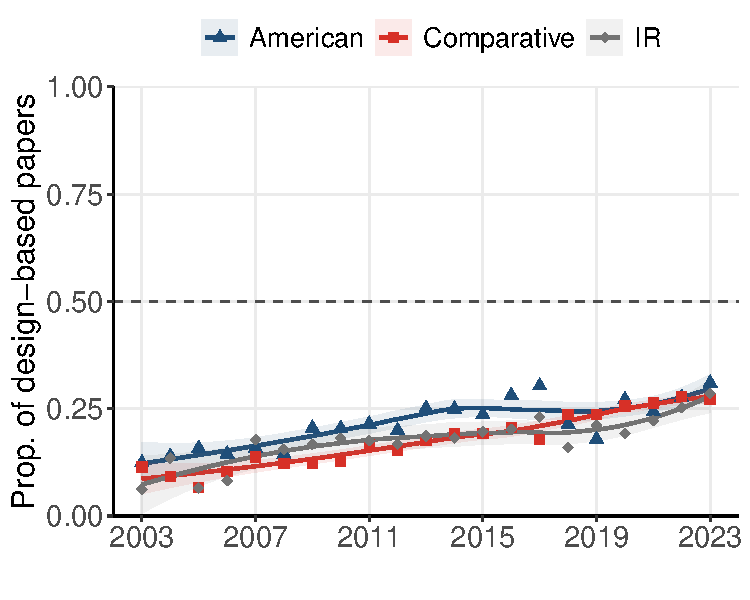
\includegraphics[width=.7\linewidth]{Figures/qe_design_subfields_shapes_nosurveys.pdf}
    \caption{Trends in the proportion of empirical quantitative papers coded as ``descriptive''.}
    \label{fig:descptrends}
\end{figure}


\begin{figure}[!ht]
    \centering
        \centering
        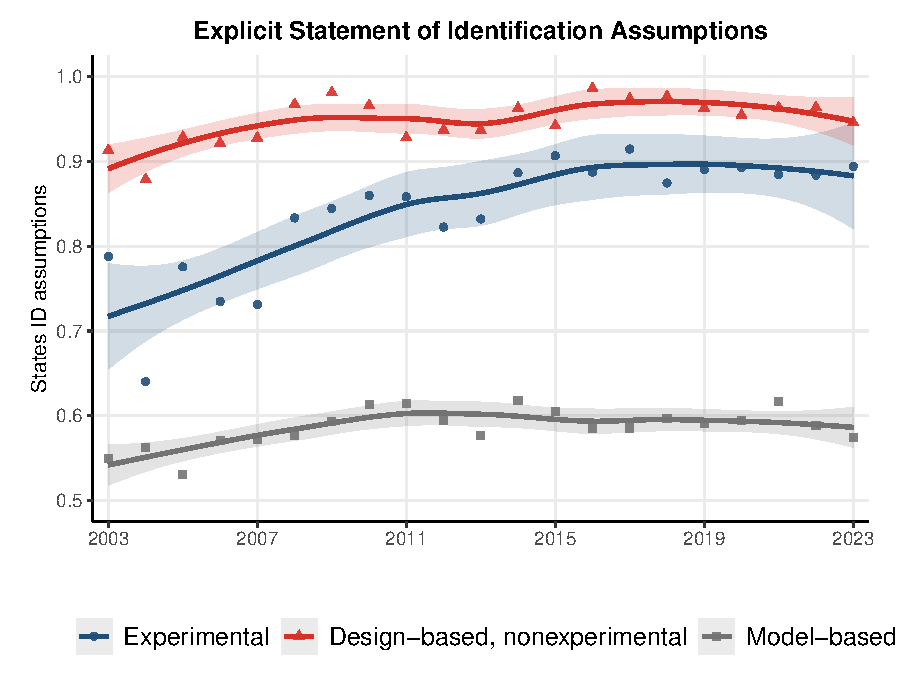
\includegraphics[width=.8\linewidth]{Figures/qe_id_assumptions.pdf}
    \caption{Trends in the proportion of explanatory papers which explicitly mention or discuss identification assumptions.}
    \label{fig:idassumps}
\end{figure}



\clearpage
\subsubsection*{Results without Survey Experiments}

While survey experiments rely on exogenous variation in the treatment assignment and consequently can be considered design-based strategies, they simultaneously could be conceptualized as measuring strategies, which spring from a different epistemological tradition. Consequently, we report results that disaggregate survey experiments from the rest of the design-based strategies in this section .

Figure~\ref{fig:basictrends_nosurvey} replicates the analysis from Figure~\ref{fig:basictrends} after excluding survey experiments from the sample. Panel (a) shows that design-based methods account for a smaller share of quantitative research under this restriction, rising from 12\% in 2003 to 27\% in 2023, while model-based methods remain dominant, and comprise more than half of the papers even in 2023. Panel (b) reveals that the exclusion affects subfields in a slightly heterogeneous fashion: American Politics sees the largest reduction in design-based papers (21 percentage points in 2023), followed by International Relations (15 percentage points) and Comparative Politics (11 percentage points).

\begin{figure}[!ht]
    \centering
    \begin{subfigure}[b]{0.47\textwidth}
        \centering
        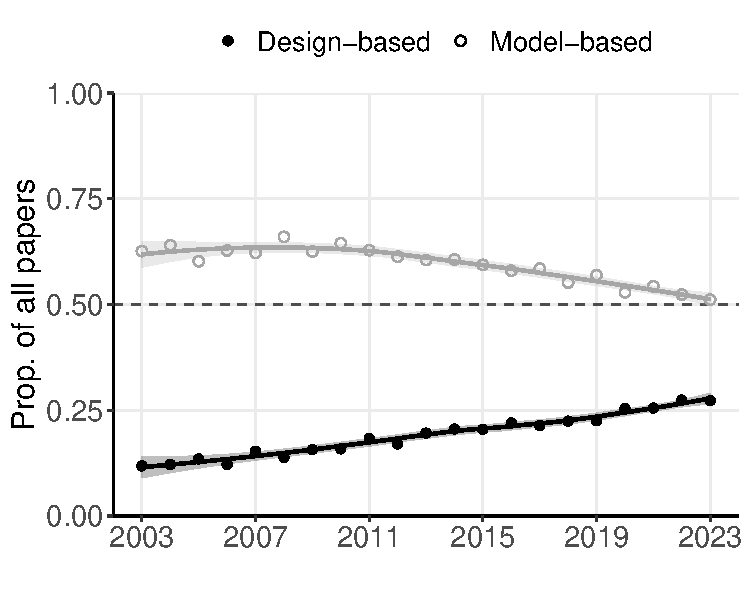
\includegraphics[width=\linewidth]{Figures/qe_design_overall_nosurveys.pdf}
        \caption{Design-based vs. model-based studies}
        \label{fig:design_overallnosurvey}
    \end{subfigure}    \hfill
    \begin{subfigure}[b]{0.47\textwidth}
        \centering
        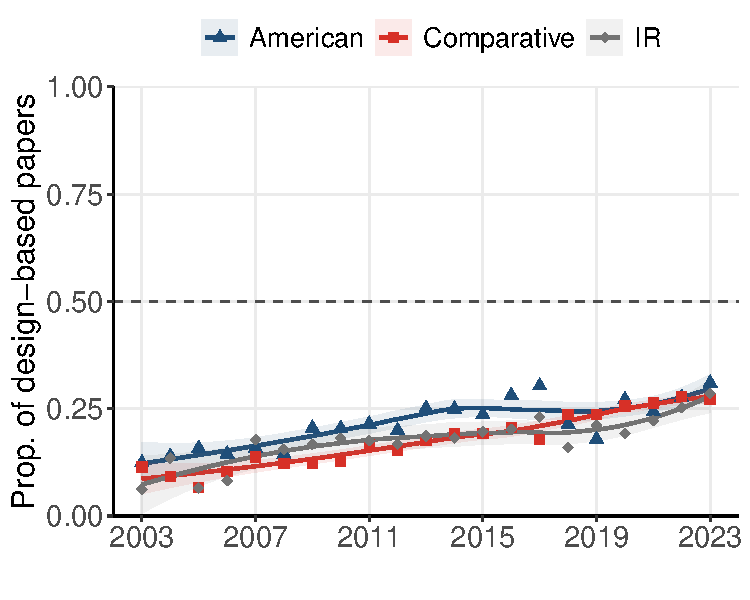
\includegraphics[width=\linewidth]{Figures/qe_design_subfields_shapes_nosurveys.pdf}
        \caption{Design-based studies by subfield}
        \label{fig:design_subfieldsnosurvey}
    \end{subfigure}

    \caption{Trends in the use of design-based methods among explanatory empirical quantitative papers when excluding survey experiments from the sample.}
    \label{fig:basictrends_nosurvey}
\end{figure}

\clearpage  
\subsubsection*{Regression Analyses}

This section presents tabular versions of selected figures from the main text. We also report a regression analysis of the citation premium associated with design-based methods, accounting for journal, subfield, and year fixed effects.



\paragraph*{Research Design Trends: Figure 5}

Table \ref{tab:design_trends} reports the data underlying Figure \ref{fig:bymethods2}, showing the distribution of research designs overall and for selected years. Design-based methods grew from 14.6\% of designs in 2003 to 40.4\% in 2023, while model-based methods declined from 60.7\% to 41.6\%.

\begin{table}[htbp]
\centering
\caption{Research design trends}
\label{tab:design_trends}
\begin{footnotesize}
\begin{tabular}{@{}lcccccccc@{}}
\toprule
Research design & \multicolumn{2}{c}{Overall} & \multicolumn{2}{c}{2003} & \multicolumn{2}{c}{2013} & \multicolumn{2}{c}{2023} \\
 & \multicolumn{2}{c}{(N=30,661)} & \multicolumn{2}{c}{(N=384)} & \multicolumn{2}{c}{(N=1,470)} & \multicolumn{2}{c}{(N=3,212)} \\
\cmidrule(lr){2-3} \cmidrule(lr){4-5} \cmidrule(lr){6-7} \cmidrule(lr){8-9}
 & N & \% & N & \% & N & \% & N & \% \\
\midrule
Model-based Methods & 15,942 & 52.0 & 233 & 60.7 & 840 & 57.1 & 1,337 & 41.6 \\
All design-based & 8,847 & 28.9 & 56 & 14.6 & 350 & 23.8 & 1,299 & 40.4 \\
\midrule
Survey Experiment & 2,964 & 9.7 & 12 & 3.1 & 75 & 5.1 & 574 & 17.9 \\
DID & 1,033 & 3.4 & 2 & 0.5 & 37 & 2.5 & 206 & 6.4 \\
Matching and Weighting & 1,340 & 4.4 & 8 & 2.1 & 68 & 4.6 & 165 & 5.1 \\
Instrumental Variable & 1,277 & 4.2 & 9 & 2.3 & 72 & 4.9 & 108 & 3.4 \\
Field Experiment & 993 & 3.2 & 14 & 3.6 & 33 & 2.2 & 98 & 3.1 \\
RDD & 395 & 1.3 & 0 & 0.0 & 12 & 0.8 & 65 & 2.0 \\
Lab Experiment & 488 & 1.6 & 7 & 1.8 & 32 & 2.2 & 35 & 1.1 \\
Natural/Quasi Experiment & 259 & 0.8 & 4 & 1.0 & 18 & 1.2 & 32 & 1.0 \\
Synthetic Control & 98 & 0.3 & 0 & 0.0 & 3 & 0.2 & 16 & 0.5 \\
\bottomrule
\end{tabular}
\end{footnotesize}
\end{table}


\paragraph*{Design-Based Share by Journal: Figure 7}

Table \ref{tab:byjournal} reports the share of design-based papers for each of the top 20 journals that underpin Figure \ref{fig:journals} in the main text, sorted by the proportion of design-based studies. Consistent with the figure, rightmost columns exclude survey experiments.

\begin{table}[htbp]
\centering
\caption{Design-based share by journal (top 20)}
\label{tab:byjournal}
\begin{tiny}
\begin{tabular}{@{}lrrccccc@{}}
\toprule
Journal & SJR rank & N & \multicolumn{2}{c}{All designs} & \multicolumn{2}{c}{Excl.\ survey exp.} \\
\cmidrule(lr){4-5} \cmidrule(lr){6-7}
 & & & \% DB & SE & \% DB & SE \\
\midrule
Quarterly Journal of Political Science & 10 & 131 & 64.9 & (0.04) & 62.0 & (0.04) \\
Political Science Research and Methods & 16 & 234 & 58.5 & (0.03) & 47.0 & (0.04) \\
American Political Science Review & 1 & 655 & 56.8 & (0.02) & 50.8 & (0.02) \\
Political Behavior & 13 & 773 & 52.7 & (0.02) & 34.9 & (0.02) \\
Public Opinion Quarterly & 19 & 336 & 52.4 & (0.03) & 28.4 & (0.03) \\
American Journal of Political Science & 2 & 973 & 47.0 & (0.02) & 39.2 & (0.02) \\
Journal of Politics & 7 & 1,348 & 45.4 & (0.01) & 36.3 & (0.01) \\
Political Communication & 18 & 339 & 43.7 & (0.03) & 27.9 & (0.03) \\
British Journal of Political Science & 9 & 655 & 37.7 & (0.02) & 28.3 & (0.02) \\
World Politics & 5 & 187 & 36.9 & (0.04) & 33.7 & (0.04) \\
International Organization & 3 & 287 & 34.1 & (0.03) & 26.6 & (0.03) \\
Journal of Conflict Resolution & 11 & 867 & 32.8 & (0.02) & 26.1 & (0.02) \\
Comparative Political Studies & 8 & 870 & 32.6 & (0.02) & 25.8 & (0.02) \\
Political Analysis & 4 & 247 & 32.4 & (0.03) & 24.1 & (0.03) \\
Journal of Peace Research & 12 & 707 & 27.2 & (0.02) & 22.5 & (0.02) \\
Journal of Public Administration Research and Theory & 6 & 482 & 26.3 & (0.02) & 19.2 & (0.02) \\
International Studies Quarterly & 15 & 740 & 24.6 & (0.02) & 17.9 & (0.01) \\
European Journal of Political Research & 14 & 613 & 21.0 & (0.02) & 14.0 & (0.01) \\
Journal of European Public Policy & 20 & 398 & 19.3 & (0.02) & 13.2 & (0.02) \\
European Union Politics & 17 & 431 & 18.1 & (0.02) & 12.2 & (0.02) \\
\bottomrule
\end{tabular}
\end{tiny}
\end{table}


\paragraph*{Citation Premium}\label{sisec:citeprem}

In Figure~\ref{fig:citemeansoverall}(b), we report evidence of a citation premium of design-based studies, relative to model-based studies. Specifically, we operationalized the measure as the difference in mean yearly citations relative to year of publication. Here we refine our measure and additionally parse out variation that could be systematically related to both method choice and citation counts to get a more fine-grained measurement of the citation premium. Specifically, we account for subfield, journal, and publication-year time invariant effects. We estimate the following regression model:
\begin{equation}
\text{Citations}_i = \beta \, D_i + \mathbf{X}_i'\boldsymbol{\gamma} + \alpha_s + \alpha_j + \alpha_t + \varepsilon_i
\end{equation}
where $D_i = 1$ if paper $i$ employs a design-based method and zero otherwise. We include fixed effects $\alpha_s$, $\alpha_j$, and $\alpha_t$ for subfields, journals, and publication year, respectively. $\mathbf{X}_i$ are author and paper-level controls, which we include in some specifications. Standard errors ($\varepsilon_i$) are clustered at the journal level.


The coefficient $\beta$ captures the average difference in citation count in 2024 for papers using a design-based method over those using a model-based method after partialing out time-invariant differences in journal popularity, subfield popularity, and year of publication. We estimate the model on the full sample and separately by cohort. The sample comprises all explanatory quantitative empirical papers in our data (2003--2023) and excludes papers classified as ``other.''

We report the results in Table \ref{tab:citation_regression}. Even-numbered columns include  $\mathbf{X}_i$---the median Shanghai ARWU rank of authors' institutions, log sample size, and a single-country indicator. On the pooled sample, design-based papers receive roughly 3.1 additional Scopus citations after accounting for fixed effects and controls (column 2, $p < 0.05$). The cohort-specific estimates reveal that this average masks substantial heterogeneity over time. In the 2007--2010 and 2011--2014 cohorts, design-based studies received approximately 11--15 additional citations ($p < 0.01$). By the 2015--2018 cohort, the estimated premium shrinks to roughly 2.5--2.9 citations and is only marginally significant. In the most recent cohort (2019--2023), the point estimates are indistinguishable from zero. While latter cohorts have had less time to accrue citations, which increase mechanically as time passes, as shown in panel a of Figure \ref{fig:citemeansoverall}, the cohort-specific results are consistent with the main findings: the citation advantage of design-based methods over model-based methods exists, sped-up, and then slowed in recent years.

\begin{table}[htbp]
\centering
\caption{Citation premium of design-based studies}
\label{tab:citation_regression}
\resizebox{\textwidth}{!}{
\begin{tabular}{lcccccccccccc}
\toprule
 & \multicolumn{2}{c}{Full sample} & \multicolumn{2}{c}{2003--2006} & \multicolumn{2}{c}{2007--2010} & \multicolumn{2}{c}{2011--2014} & \multicolumn{2}{c}{2015--2018} & \multicolumn{2}{c}{2019--2023} \\
\cmidrule(lr){2-3} \cmidrule(lr){4-5} \cmidrule(lr){6-7} \cmidrule(lr){8-9} \cmidrule(lr){10-11} \cmidrule(lr){12-13}
 & (1) & (2) & (3) & (4) & (5) & (6) & (7) & (8) & (9) & (10) & (11) & (12) \\
\midrule
Design-based & 1.70 & 3.14$^{**}$ & 13.77 & 7.84 & 10.95$^{***}$ & 15.29$^{***}$ & 8.88$^{***}$ & 11.59$^{***}$ & 2.89$^{**}$ & 2.56$^{\dagger}$ & -0.06 & 0.33 \\
 & (1.05) & (1.22) & (10.87) & (9.85) & (3.94) & (5.01) & (2.68) & (2.99) & (1.24) & (1.40) & (0.44) & (0.47) \\
\midrule
Controls & No & Yes & No & Yes & No & Yes & No & Yes & No & Yes & No & Yes \\
Subfield FE & Yes & Yes & Yes & Yes & Yes & Yes & Yes & Yes & Yes & Yes & Yes & Yes \\
Journal FE & Yes & Yes & Yes & Yes & Yes & Yes & Yes & Yes & Yes & Yes & Yes & Yes \\
Year FE & Yes & Yes & Yes & Yes & Yes & Yes & Yes & Yes & Yes & Yes & Yes & Yes \\
\midrule
Observations & 24,558 & 16,966 & 1,467 & 932 & 3,213 & 2,118 & 4,593 & 2,989 & 5,354 & 3,686 & 9,931 & 7,241 \\
$R^2$ & 0.203 & 0.213 & 0.219 & 0.312 & 0.142 & 0.167 & 0.155 & 0.157 & 0.158 & 0.149 & 0.162 & 0.201 \\
Adj.\ $R^2$ & 0.197 & 0.206 & 0.171 & 0.242 & 0.112 & 0.123 & 0.131 & 0.121 & 0.136 & 0.118 & 0.150 & 0.186 \\
\bottomrule
\end{tabular}
}
\vspace{0.3em}
\begin{minipage}{\textwidth}
\footnotesize
\textit{Notes:} $^{***}p<0.01$, $^{**}p<0.05$, $^{\dagger}p<0.1$.
Standard errors clustered by journal in parentheses. Controls: median Shanghai ARWU rank of authors' institutions, log sample size, and single-country indicator. Sample restricted to design-based and model-based papers.
\end{minipage}
\end{table}
\clearpage

\subsubsection*{Other results}

In the main text, we argue and show evidence of design-based research being adopted heterogeneously in the discipline across journals and institutions. Consequently, in Figure~\ref{fig:linestopjournals} we show which specific design-based methods are driving the methodological shift and how these patterns differ between top journals and the rest of the field. It compares the prevalence of each method in the top 20 journals versus all other outlets. With most design-based methods, top journals adopt design-based strategies earlier and at higher rates, indicating that influential outlets play a disproportionate role in shaping the trajectory of causal inference practices in the discipline. Overall, the figure highlights that the credibility revolution has been propelled largely by a small set of design-based methods, especially survey experiments and difference-in-differences, with high-impact journals consistently at the leading edge of this shift.


\begin{figure}[!ht]
    \centering

    \begin{subfigure}[b]{0.95\textwidth}
        \centering
        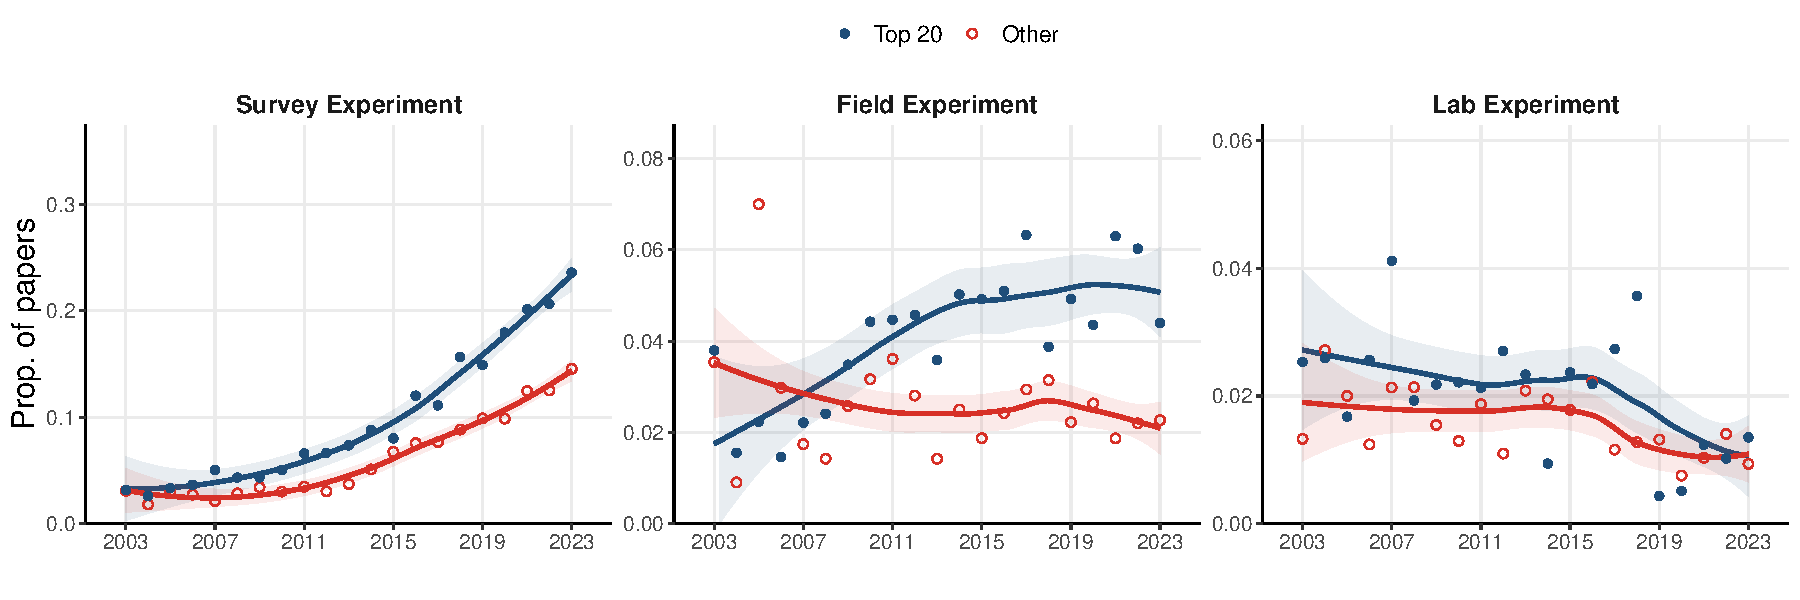
\includegraphics[width=\linewidth]{Figures/qrd2_lines_topjournals_rd_experiments.pdf}
        \caption{Experimental}
        \label{fig:experimentslinestop20}
    \end{subfigure}
    \hfill
    \begin{subfigure}[b]{0.95\textwidth}
        \centering
        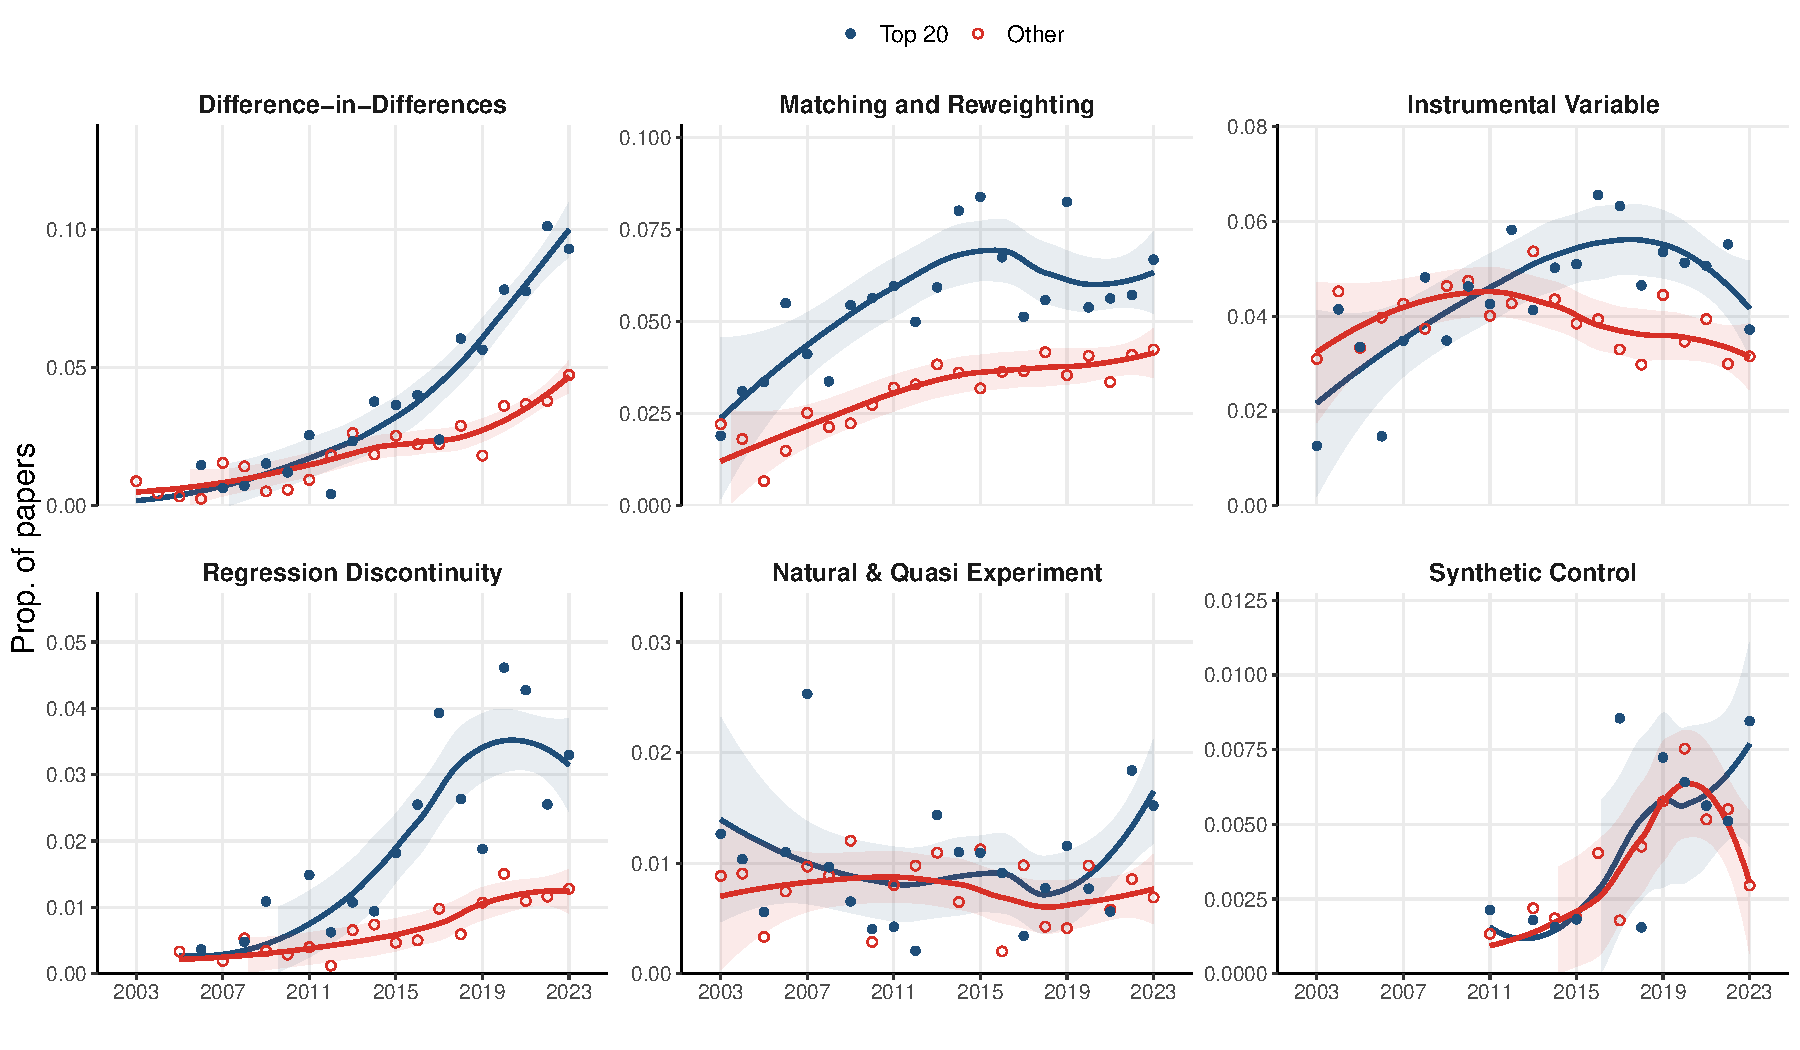
\includegraphics[width=\linewidth]{Figures/qrd2_lines_topjournals_rd_nonexperiments.pdf}
        \caption{Non-experimental}
        \label{fig:notexperimentslinestop20}
    \end{subfigure}
\caption{Proportion of each design-based method by journal ranking and year. The denominator is the total number of explanatory empirical quantitative studies published each year. Top 20 journals are shown in blue; all other journals in red.}
    \label{fig:linestopjournals}
\end{figure}


\end{document}
